%\documentclass[1p]{elsarticle}
\documentclass[review]{elsarticle}

\usepackage{lineno,hyperref}
\usepackage{amsfonts}
\usepackage{amsmath}
\usepackage{amssymb}
\usepackage{amsthm}
\usepackage{mathrsfs}
\usepackage{subcaption}
\usepackage{float}

\modulolinenumbers[5]
\hypersetup{
  bookmarksnumbered = true,
  bookmarksopen=false,
  pdfborder=0 0 0,         % make all links invisible, so the pdf looks good when printed
  pdffitwindow=true,      % window fit to page when opened
  pdfnewwindow=true, % links in new window
  colorlinks=true,           % false: boxed links; true: colored links
  linkcolor=blue,            % color of internal links
  citecolor=magenta,    % color of links to bibliography
  filecolor=magenta,     % color of file links
  urlcolor=cyan              % color of external links
}


\journal{Journal of Computational Physics}

%%%%%%%%%%%%%%%%%%%%%%%
%% Elsevier bibliography styles
%%%%%%%%%%%%%%%%%%%%%%%
%% To change the style, put a % in front of the second line of the current style and
%% remove the % from the second line of the style you would like to use.
%%%%%%%%%%%%%%%%%%%%%%%

%% Numbered
%\bibliographystyle{model1-num-names}

%% Numbered without titles
%\bibliographystyle{model1a-num-names}

%% Harvard
%\bibliographystyle{model2-names.bst}\biboptions{authoryear}

%% Vancouver numbered
%\usepackage{numcompress}\bibliographystyle{model3-num-names}

%% Vancouver name/year
%\usepackage{numcompress}\bibliographystyle{model4-names}\biboptions{authoryear}

%% APA style
%\bibliographystyle{model5-names}\biboptions{authoryear}

%% AMA style
%\usepackage{numcompress}\bibliographystyle{model6-num-names}

%% `Elsevier LaTeX' style
\bibliographystyle{elsarticle-num}
%%%%%%%%%%%%%%%%%%%%%%%

\newtheorem{define}{Definition}
\newtheorem{lemma}{Lemma}
\newtheorem{prop}{Proposition}
\newtheorem{rem}{Remark}
\newtheorem{theorem}{Theorem}

%\newcommand{\ee}[1]{{\color{red} EE:~#1}}
%\newcommand{\rc}[1]{{\color{blue} RC:~#1}}

\newcommand{\modified}[1]{{\color{red}#1}}

\usepackage{./definitions}

\begin{document}

\begin{frontmatter}

\title{Realizability-Preserving DG-IMEX Method for the Two-Moment Model of Fermion Transport \tnoteref{support}\tnoteref{copyright}}
\tnotetext[support]{
This research is sponsored, in part, by the Laboratory Directed Research and Development Program of Oak Ridge National Laboratory (ORNL), managed by UT-Battelle, LLC for the U. S. Department of Energy under Contract No. De-AC05-00OR22725.  
This research was supported by the Exascale Computing Project (17-SC-20-SC), a collaborative effort of the U.S. Department of Energy Office of Science and the National Nuclear Security Administration.  
This material is based, in part, upon work supported by the U.S. Department of Energy, Office of Science, Office of Advanced Scientific Computing Research.  
Eirik Endeve was supported in part by NSF under Grant No. 1535130.}
\tnotetext[copyright]{
This manuscript has been authored by UT-Battelle, LLC under Contract No. DE-AC05-00OR22725 with the U.S. Department of Energy. The United States Government retains and the publisher, by accepting the article for publication, acknowledges that the United States Government retains a non-exclusive, paid-up, irrevocable, world-wide license to publish or reproduce the published form of this manuscript, or allow others to do so, for United States Government purposes. The Department of Energy will provide public access to these results of federally sponsored research in accordance with the DOE Public Access Plan(http://energy.gov/downloads/doe-public-access-plan).}

%% Group authors per affiliation:
\author[utk-phys]{Ran Chu}
\ead{rchu@vols.utk.edu}

\author[ornl,utk-phys,jics]{Eirik Endeve\corref{cor}}
\ead{endevee@ornl.gov}

\author[ornl,utk-math]{Cory D. Hauck}
\ead{hauckc@ornl.gov}

\author[utk-phys,jics]{Anthony Mezzacappa}
\ead{mezz@utk.edu}

\cortext[cor]{Corresponding author. Tel.:+1 865 576 6349; fax:+1 865 241 0381}

\address[ornl]{Computational and Applied Mathematics Group, Oak Ridge National Laboratory, Oak Ridge, TN 37831 USA }

\address[utk-phys]{Department of Physics and Astronomy, University of Tennessee Knoxville, TN 37996-1200}

\address[jics]{Joint Institute for Computational Sciences, Oak Ridge National Laboratory, Oak Ridge, TN 37831-6354}

\address[utk-math]{Department of Mathematics, University of Tennessee Knoxville, TN 37996-1320}

\begin{abstract}
Building on the framework of Zhang \& Shu \cite{zhangShu_2010a,zhangShu_2010b}, we develop a realizability-preserving method to simulate the transport of particles (fermions) through a background material using a two-moment model that evolves the angular moments of a phase space distribution function $f$.  
The two-moment model is closed using algebraic moment closures; e.g., as proposed by Cernohorsky \& Bludman \cite{cernohorskyBludman_1994} and Banach \& Larecki \cite{banachLarecki_2017a}.  
Variations of this model have recently been used to simulate neutrino transport in nuclear astrophysics applications, including core-collapse supernovae and compact binary mergers.  
We employ the discontinuous Galerkin (DG) method for spatial discretization (in part to capture the asymptotic diffusion limit of the model) combined with implicit-explicit (IMEX) time integration to stably bypass short timescales induced by frequent interactions between particles and the background.  
Appropriate care is taken to ensure the method preserves strict algebraic bounds on the evolved moments (particle density and flux) as dictated by Pauli's exclusion principle, which demands a bounded distribution function (i.e., $f\in[0,1]$).  
This realizability-preserving scheme combines a suitable CFL condition, a realizability-enforcing limiter, a closure procedure based on Fermi-Dirac statistics, and an IMEX scheme whose stages can be written as a convex combination of forward Euler steps combined with a backward Euler step.  
The IMEX scheme is formally only first-order accurate, but works well in the diffusion limit, and --- without interactions with the background --- reduces to the optimal second-order strong stability-preserving explicit Runge-Kutta scheme of Shu \& Osher \cite{shuOsher_1988}.  
Numerical results demonstrate the realizability-preserving properties of the scheme.  
We also demonstrate that the use of algebraic moment closures not based on Fermi-Dirac statistics can lead to unphysical moments in the context of fermion transport.  
\end{abstract}

\begin{keyword}
Boltzmann equation, 
Radiation transport, 
Hyperbolic conservation laws, 
Discontinuous Galerkin, 
Implicit-Explicit, 
Moment Realizability
\end{keyword}

\end{frontmatter}

\tableofcontents

\linenumbers

\section{Introduction}

Core-collapse supernovae (CCSNe) are the explosion happens at the end of a massive star's life.
They are a dominant source of heavy elements and play an important role in many astrophysical phenomena, such as neutron star and black hole formation.  
Furthermore, these explosions occur at energies and densities relevant to address fundamental questions in nuclear, particle, and gravitational physics. 
A solid theoretical framework for these explosion mechanism will illuminate explanations to many import questions in fundamental physics.

One essential part of the explosion mechanism is neutrino transport which drives the explosion.  
Neutrino transport is modeled by Boltzmann transport equation, which is partial differential equation and evolves the distribution function $f$.
Simulating the neutrino transport is finding a solution of Boltzmann transport equation for a given domain and period with an acceptable accuracy.

Solving Boltzmann transport multi-dimensional with high accuracy requirement can be expensive.
\ee{Balance physical fidelity and computational expediency?}
One alternation is sacrificing the accuracy: instead of solving Boltzmann transport equations, solve moment equation for an approximate solution.
\ee{What are moments?}
This kind method is moment method and we focus on two-moment method in this paper.

Applying two-moment method only is not sufficient to have an affordable solution when the simulating period is long.
To be precisely, neutrino interact with the background rapidly and its characteristic time scalar is so small comparing to the length of CCSNe explosion process. 
It makes the time step needed by an explicit time integrator dramatic small and a huge mount of calculation needed. 
\ee{Discuss fully implicit approach?}
To manipulate this challenge, implicit-explicit (IMEX) methods are taken into consideration.
By taking advantage of the fact that collision terms are local, IMEX methods are able to make the time integrator more efficient in diffusion dominate region.

However, price needs to be paid for the lunch.  
\ee{Nonlinear equations, closure, well-posedness of closure requires realizable moments}
\ee{What is moment realizability}
Two-moment method requires a realizability-preserving algebraic closure for fermion.
IMEX methods should be diffusion limit accurate \ee{why?}. 
The discussion of these prices drives this paper. 
\ee{Moment realizabilty and diffusion accurate IMEX scheme motivates this work}

This paper is recognized as following: Section~\ref{se:Two-MomentModel} discusses the mathematical model, algebraic closures, and realizability algebraic closures in the context of Fermi-Dirac statistics;
Section~\ref{se:SpacialDiscretization} we discuss moment realizability in the context of a first-order finite volume spatial discretization; Section~\ref{se:TimeIntegration} discusses how to construct a constraint-preserving, diffusion limit accurate IMEX (PD-ARS) scheme and two PD-ARS schemes are presented \ee{should we introduce the term PD-ARS here?}; Section~\ref{se:NumericalTests} gives the result of the numerical tests of the PD-ARSs; Section~\ref{se:Conclusion} is the conclusion section.
\section{Mathematical Model}
\label{sec:model}

In this section we give a summary of the mathematical model.  

\subsection{Boltzmann Equation}

We consider approximate solutions to the Boltzmann equation for the transport of massless particles through a static material in Cartesian geometry, which, after scaling to dimensionless units, can be written as
\begin{equation}
  \pd{f}{t}+\vect{\ell}\cdot\nabla f
  =\f{1}{\tau}\,\cC(f),
  \label{eq:boltzmann}
\end{equation}
where the distribution function $f\colon(\omega,\varepsilon,\vect{x},t)\in\bbS^{2}\times\bbR^{+}\times\bbR^{3}\times\bbR^{+}\to\bbR^{+}$ gives the number of particles propagating in the direction $\omega\in\bbS^{2}:=\{\,\omega=(\thetaNu,\phiNu)~|~\thetaNu\in[0,\pi],\phiNu\in[0,2\pi)\,\}$, with energy $\varepsilon\in\bbR^{+}$, at position $\vect{x}\in\bbR^{3}$ and time $t\in\bbR^{+}$.  
Here we use spherical momentum space coordinates $(\varepsilon,\omega)$, and the unit vector $\vect{\ell}(\omega)\in\bbR^{3}$ (independent of $\varepsilon$ and $\vect{x}$) is parallel to the particle three-momentum $\vect{p}=\varepsilon\,\vect{\ell}$.  
We also define the energy-position coordinates $\vect{z}:=\{\varepsilon,\vect{x}\}\in\bbR^{+}\times\bbR^{3}$.  
On the right-hand side of Eq.~\eqref{eq:boltzmann}, $\tau$ is the ratio of the particle mean-free path (due to interactions with a background) to some characteristic length scale of the problem.  
In opaque regions, $\tau\ll1$, while for free streaming particles, $\tau\gg1$.  
The collision operator, which models emission, absorption, and isotropic and elastic scattering, is given by
\begin{equation}
  \cC(f)=\xi\,\big(\,f_{0}-f\,\big)
  +(1-\xi)\,\big(\,\f{1}{4\pi}\int_{\bbS^{2}}f\,d\omega-f\,\big),
  \label{eq:collisionTerm}
\end{equation}
where $\xi=\sigma_{\Ab}/\sigma_{\Tot}\in[0,1]$ is the ratio of the absorption opacity $\sigma_{\Ab}\,(\ge0)$ to the total opacity $\sigma_{\Tot}=\sigma_{\Ab}+\sigma_{\Scatt}$, and $\sigma_{\Scatt}\,(\ge0)$ is the scattering opacity.  
In particular, $\xi=1$ models pure emission and absorption, while $\xi=0$ models pure scattering.  
In general, $\sigma_{\Ab}$ and $\sigma_{\Scatt}$ (and $\tau$ and $\xi$) depend on $\vect{z}$.  
The equilibrium distribution function is denoted by $f_{0}(\vect{z})$.  
Here, we consider transport of Fermions (e.g., neutrinos), so the equilibrium distribution function takes the form
\begin{equation}
  f_{0}(\vect{z})=\f{1}{e^{(\varepsilon-\mu(\vect{x}))/T(\vect{x})}+1},  
  \label{eq:fermiDirac}
\end{equation}
where the temperature $T$ and the chemical potential $\mu$ depend on properties of the background.  

\subsection{Angular Moment Equations: Two-Moment Model}

The Boltzmann equation is often too expensive to solve directly.  
Instead, approximate equations for angular moments of the distribution function are solved.  
To this end, we define the angular moments of the distribution function
\begin{equation}
  \big\{\,\cJ,\vect{\cH},\vect{\cK}\,\big\}(\vect{z},t)
  =\f{1}{4\pi}\int_{\bbS^{2}}f(\omega,\vect{z},t)\,\{\,1,\vect{\ell},\vect{\ell}\otimes\vect{\ell}\,\}\,d\omega.  
  \label{eq:angularMoments}
\end{equation}
We refer to $\cJ$ (zeroth moment) as the particle density, $\vect{\cH}$ (first moment) as the particle flux, and $\vect{\cK}$ (second moment) as the stress tensor.  
Note that the moments defined in Eq.~\eqref{eq:angularMoments} are \emph{spectral moments} (depending on energy as well as position and time).  
The \emph{grey moments} (depending only on position and time) are obtained by integration over energy:
\begin{equation}
  \big\{\,J,\vect{H},\vect{K}\,\big\}(\vect{x},t)
  =\int_{\bbR^{+}}\big\{\,\cJ,\vect{\cH},\vect{\cK}\,\big\}(\varepsilon,\vect{x},t)\,\varepsilon^{2}d\varepsilon.  
\end{equation}

Taking the zeroth and first moments of Eq.~\eqref{eq:boltzmann} gives the two-moment model, comprising a system of conservation laws with sources
\begin{equation}
  \pd{\vect{\cM}}{t}+\nabla\cdot\vect{\cF}=\f{1}{\tau}\,\vect{\cC}(\vect{\cM}),
  \label{eq:momentEquations}
\end{equation}
where $\vect{\cM}=(\cJ,\vect{\cH})^{T}$ and $\vect{\cF}=(\vect{\cH},\vect{\cK})^{T}$.  
Components of the fluxes in each coordinate direction are $\vect{\cF}^{i}=\vect{e}_{i}\cdot\vect{\cF}=(\vect{e}_{i}\cdot\vect{\cH},\vect{e}_{i}\cdot\vect{\cK})^{T}$, where $\vect{e}_{i}$ is the unit vector parallel to the $i$th coordinate direction.  
On the right-hand side of Eq.~\eqref{eq:momentEquations}, the source term is
\begin{equation}
  \vect{\cC}(\vect{\cM})=\vect{\eta}-\vect{\cD}\,\vect{\cM}, 
  \label{eq:collisionTermMoments}
\end{equation}
where $\vect{\eta}=(\xi\,f_{0},\vect{0})^{T}$ and $\vect{\cD}=\mbox{diag}(\xi,\vect{I})$, with $\vect{I}$ the identity matrix.  

In order to close the system given by Eq.~\eqref{eq:momentEquations}, the components of the stress tensor $\vect{\cK}$ must be related to the lower moments through a closure procedure.  
To this end, Levermore \cite{levermore_1984} defined the Eddington tensor $\vect{k}=\vect{\cK}/\cJ$ and assumed that the radiation field is symmetric about a preferred direction $\widehat{\vect{h}}=\vect{\cH}/|\vect{\cH}|$ so that
\begin{equation}
  \vect{k}=\f{1}{2}\big[\,\big(1-\chi\big)\,\vect{I}+\big(3\,\chi-1\big)\,\widehat{\vect{h}}\otimes\widehat{\vect{h}}\,\big],
  \label{eq:eddingtonTensor}
\end{equation}
where $\chi=\chi(\cJ,|\vect{\cH}|)$ is the Eddington factor.  
The two-moment model is then closed once the Eddington factor is determined from $\cJ$ and $\vect{\cH}$.  
We will return to the issue of determining the Eddington factor in Section~\ref{sec:algebraicClosure}.  
\section{Moment Realizability for the Fermionic Two-Moment Model}
\label{sec:realizability}

Our goal is to simulate massless fermions (e.g., neutrinos) and study their interactions with matter.  
The principal objective is to obtain the fermionic distribution function $f$ (or moments of $f$ as in the two-moment model employed here).  
The Pauli exclusion principle requires the distribution function to satisfy the condition $0 \le f \le 1$, which puts restrictions on the admissible values for the moments of $f$.  
In this paper, we seek to design a numerical method for solving the system of moment equations given by Eq.~\eqref{eq:momentEquations} that preserves realizability of the moments; i.e., the moments evolve within the set of admissible values as dictated by Pauli's exclusion principle.  
(Since we are only concerned with the angular dependence of $f$ in this section, we simplify the notation by suppressing the $\vect{z}$ and $t$ dependence and write $f(\omega,\vect{z},t)=f(\omega)$.)  

We begin with the following definition of moment realizability.  
\begin{define}
  The moments $\vect{\cM}=\big(\cJ,\vect{\cH}\big)^{T}$ are realizable if they can be obtained from a distribution function satisfying $0 < f(\omega) < 1~\forall~\omega\in\bbS^{2}$.
  \label{def:momentRealizability}
\end{define}
\begin{rem}
  Following \cite{lareckiBanach_2011}, in Definition~\ref{def:momentRealizability}, and in the rest of this paper, we exclude the cases $f=0$ and $f=1$ almost everywhere (a.e.) on $\bbS^{2}$, which would give $\cJ=0$, $\vect{\cH}=0$ and $\cJ=1$, $\vect{\cH}=0$, respectively.  
\end{rem}

Realizable moments satisfy algebraic constraints.  
We proceed by stating the constraints on the moments by restating results from Theorem~7.1 in \cite{banachLarecki_2017a} in the following Lemma.  
The proof is given in \cite{banachLarecki_2017a}.  
(See also \cite{lareckiBanach_2011,banachLarecki_2013}.)
\begin{lemma}
  Suppose that $0 < f(\omega) < 1~\forall~\omega\in\bbS^{2}$.  
  Then the moments $\vect{\cM}=(\cJ,\vect{\cH})^{T}$, defined as in Eq.~\eqref{eq:angularMoments}, satisfy $0 < \cJ < 1$ and $\big(1-\cJ\big)\,\cJ-|\vect{\cH}| > 0$. 
  \label{lem:MomentRealizable} 
\end{lemma}

\begin{define}
  For the fermion two-moment model, the realizable set is
  \begin{equation}
    \cR:=\big\{\,\vect{\cM}=\big(\cJ,\vect{\cH}\big)^{T}~|~\cJ\in(0,1)~\text{and}~\gamma(\vect{\cM})\equiv(1-\cJ)\cJ-|\vect{\cH}| > 0\,\big\}.
    \label{eq:realizableSet}
  \end{equation}
\end{define}

\begin{lemma}
  The realizable set $\cR$, defined in Eq.~\eqref{eq:realizableSet}, is convex.  
\end{lemma}
\begin{proof}
  In order to prove that $\cR$ is convex, it is sufficient to show that any convex combination of elements in $\cR$ also belongs to $\cR$.  
  Let $\vect{\cM}_{a}=\big(\cJ_{a},\vect{\cH}_{a}\big)^{T}$ and $\vect{\cM}_{b}=\big(\cJ_{b},\vect{\cH}_{b}\big)^{T}$ be two arbitrary elements in $\cR$.  
  Consider the convex combination $\vect{\cM}_{c} = \theta\,\vect{\cM}_{a} + (1-\theta)\,\vect{\cM}_{b}$, with $0\leq\theta\leq1$.
  The first component of $\vect{\cM}_{c}$ is
  \begin{equation*}
    \cJ_{c} = \theta\,\cJ_{a} + (1-\theta)\,\cJ_{b}.
  \end{equation*}
  Since $\cJ_{a},\cJ_{b} \in (0,1)$, it follows that $\cJ_{c} \in (0,1)$.  
  Since $\cJ_{a},\cJ_{b} \in (0,1)$, it is straightforward to verify that
  \begin{equation*}
  \gamma(\vect{\cM}_{c}) \geq \theta\,\gamma(\vect{\cM}_{a}) + (1-\theta)\,\gamma(\vect{\cM}_{b}) > 0.
  \end{equation*}
  Hence, $\vect{\cM}_{c}\in\cR$.
\end{proof}

Figure~\ref{fig:RealizableSetFermionic} illustrates the geometry of the convex set $\cR$ in the $(\cH,\cJ)$-plane (light blue region).  
The boundary $\partial\cR$ (black curves) is given by $\gamma(\vect{\cM})=0$.  
The realizable domain of positive distribution functions, $\cR^{+}$ (no upper bound on $f$), which is a convex cone defined by
\begin{equation}
  \cR^{+}:=\big\{\,\vect{\cM}=\big(\cJ,\vect{\cH}\big)^{T}~|~\cJ > 0~\text{and}~\cJ > |\vect{\cH}|\,\big\}, 
  \label{eq:realizableSetPositive}
\end{equation}
is partially shown as the light red region above the red lines, which mark the boundary of $\cR^{+}$ (denoted $\partial\cR^{+}$).  
(A realizability-preserving method, with respect to $\cR^{+}$, for the two-moment model in one spatial dimension was developed in \cite{olbrant_etal_2012}.)  
The realizable domains $\cR$ and $\cR^{+}$ overlap for low particle densities ($\cJ\ll1$), but for larger values of $\cJ$, the realizable domain of particles governed by Fermi-Dirac statistics is much more restricted than that of particles described by positive distribution functions with no upper bound.  

\begin{figure}[H]
  \centering
  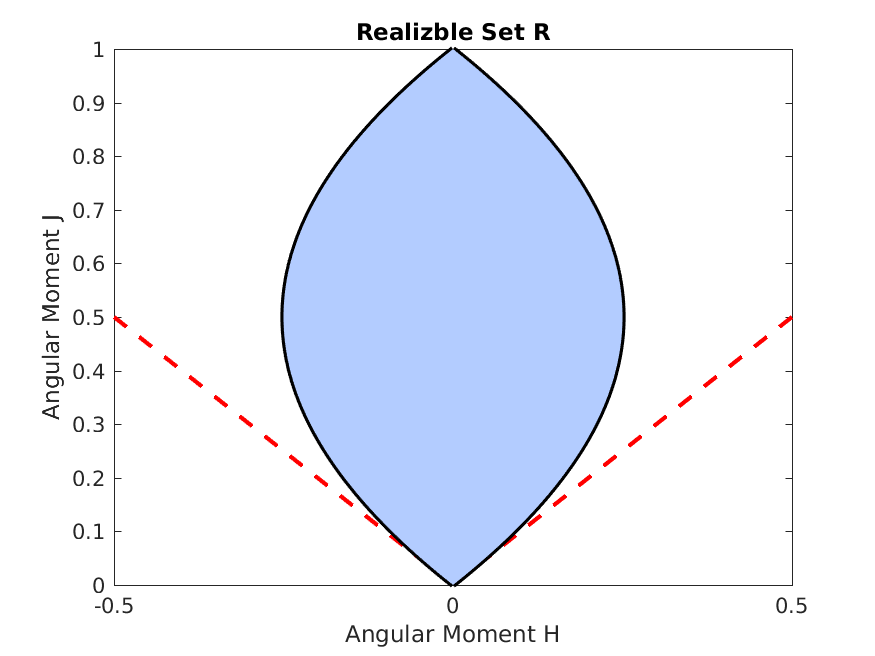
\includegraphics[width=1.0\linewidth]{figures/RealizableSetFermionic}
  \caption{Illustration of the realizable set $\cR$ (light blue region) defined in Eq.~\eqref{eq:realizableSet}.  
  The black lines define the boundary $\partial\cR$, while the red lines indicate the boundary of the realizable set $\cR^{+}$ (light red region) defined in Eq.~\eqref{eq:realizableSetPositive}.}
  \label{fig:RealizableSetFermionic}
\end{figure}

For the realizability-preserving scheme developed in Section~\ref{sec:realizableDGIMEX}, we state some additional results.  
Lemma~\ref{lem:explicitStep} is used to help prove the realizability-preserving property of explicit steps in the IMEX scheme, while Lemmas~\ref{lem:implicitStep} and \ref{lem:correctionStep} are used to prove realizability-preserving properties of implicit steps.  
\begin{lemma}
  Let $\big\{\cJ_{a},\vect{\cH}_{a},\vect{\cK}_{a}\big\}$ and $\big\{\cJ_{b},\vect{\cH}_{b},\vect{\cK}_{b}\big\}$ be moments defined as in Eq.~\eqref{eq:angularMoments} with distribution functions $f_{a}$ and $f_{b}$, respectively, such that $f_{a}(\omega),f_{b}(\omega)\in(0,1)\,\forall\,\omega\in\bbS^{2}$.  
  Let $\Phi^{\pm}(\vect{\cM},\vect{\cK})=\f{1}{2}\big(\vect{\cM}\pm\widehat{\vect{e}}\cdot\vect{\cF}\big)$, where $\widehat{\vect{e}}\in\bbR^{3}$ is an arbitrary unit vector, and $\widehat{\vect{e}}\cdot\vect{\cF}=\big(\widehat{\vect{e}}\cdot\vect{\cH},\widehat{\vect{e}}\cdot\vect{\cK}\big)^{T}$.  
  Then
  \begin{equation*}
    \vect{\cM}_{ab} = \big(\cJ_{ab},\vect{\cH}_{ab}\big)^{T} \equiv \Phi^{+}(\vect{\cM}_{a},\vect{\cK}_{a})+\Phi^{-}(\vect{\cM}_{b},\vect{\cK}_{b})\in\cR.
  \end{equation*}
  \label{lem:explicitStep}
\end{lemma}
\begin{proof}
  It is straightforward to rewrite the components of $\vect{\cM}_{ab}$ as
  \begin{equation*}
    \cJ_{ab}=\f{1}{4\pi}\int_{\bbS^{2}}f_{ab}(\omega)\,d\omega
    \quad\text{and}\quad
    \vect{\cH}_{ab}=\f{1}{4\pi}\int_{\bbS^{2}}f_{ab}(\omega)\,\vect{\ell}(\omega)\,d\omega,
  \end{equation*}
  where $f_{ab}(\omega)=\vartheta\,f_{a}(\omega)+(1-\vartheta)\,f_{b}(\omega)$ and $\vartheta(\omega)=(1+\widehat{\vect{e}}\cdot\vect{\ell}(\omega))/2\in[0,1]$.  
  Then, since $f_{ab}(\omega)\in(0,1)\,\forall\,\omega\in\bbS^{2}$, we have from Lemma~\ref{lem:MomentRealizable} that $\vect{\cM}_{ab}\in\cR$.  
\end{proof}

\begin{lemma}
  Let $\vect{\cM}_{a}=(\cJ_{a},\vect{\cH}_{a})^{T}\in\cR$ and $\alpha>0$.  
  Let $\vect{\cM}_{b}=(\cJ_{b},\vect{\cH}_{b})^{T}$ satisfy
  \begin{equation*}
    \vect{\cM}_{b}=\vect{\cM}_{a}+\alpha\,\vect{\cC}(\vect{\cM}_{b}), 
  \end{equation*}
  where $\vect{\cC}(\vect{\cM})=\vect{\eta}-\vect{\cD}\,\vect{\cM}$ is the collision term in Eq.~\eqref{eq:collisionTermMoments}.  
  Then $\vect{\cM}_{b}\in\cR$.  
  \label{lem:implicitStep}
\end{lemma}
\begin{proof}
  Solving for $\vect{\cM}_{b}$ gives $\vect{\cM}_{b} = \big(\vect{I}+\alpha\,\vect{\cD}\big)^{-1}\big(\vect{\cM}_{a}+\alpha\,\vect{\eta}\big)$.  
  The first component of $\vect{\cM}_{b}$ can be written as
  \begin{equation*}
    \cJ_{b}=\f{1}{4\pi}\int_{\bbS}f_{b}(\omega)\,d\omega,
  \end{equation*}
  where $f_{b}(\omega)=\zeta\,f_{a}(\omega)+(1-\zeta)\,f_{0}$, $\zeta=1/(1+\alpha\,\xi)\in[0,1]$, and $f_{0}$ and $\xi$ are defined in Section~\ref{sec:model}.  
  Then, since $f_{b}(\omega)\in(0,1)\,\forall\,\omega\in\bbS^{2}$, $\cJ_{b}\in(0,1)$.  
  Similarly, we can write
  \begin{equation*}
    \vect{\cH}_{b}=\f{(1+\alpha\,\xi)}{(1+\alpha)}\,\widetilde{\vect{\cH}}_{b},
    \quad\text{where}\quad
    \widetilde{\vect{\cH}}_{b}=\f{1}{4\pi}\int_{\bbS^{2}}f_{b}(\omega)\,\vect{\ell}(\omega)\,d\omega.  
  \end{equation*}
  It follows from Lemma~\ref{lem:MomentRealizable} that $\widetilde{\vect{\bcM}}_{b}=(\cJ_{b},\widetilde{\vect{\cH}}_{b})^{T}\in\cR$.  
  Then, since $0\le\xi\le1$, we have $|\vect{\cH}_{b}|\le|\widetilde{\vect{\cH}}_{b}| < (1-\cJ_{b})\,\cJ_{b}$.  
\end{proof}

\begin{lemma}
  Let $\vect{\cM}_{a}$ and $\alpha$ be given as in Lemma~\ref{lem:implicitStep}, and let $\vect{\cM}_{b}$ satisfy
  \begin{equation*}
    \vect{\cM}_{b}=\vect{\cM}_{a}+\alpha\,\vect{\cD}\,\vect{\cC}(\vect{\cM}_{b}),    
  \end{equation*}
  where $\vect{\cD}$ and $\vect{\cC}(\vect{\cM})$ are given by Eq.~\eqref{eq:collisionTermMoments},  then $\vect{\cM}_{b}\in\cR$.  
  \label{lem:correctionStep}
\end{lemma}
The proof of Lemma~\ref{lem:correctionStep} follows along the same lines as the proof of Lemma~\ref{lem:implicitStep} and is omitted.  

\section{Algebraic Moment Closures}
\label{sec:algebraicClosure}

The two-moment model given by Eq.~\eqref{eq:angularMoments} is not closed because of the appearance of the second moments $\vect{\cK}$ (the normalized pressure tensor).  
Algebraic moment closures for the two-moment model are computationally efficient as they provide the Eddington factor in Eq.~\eqref{eq:eddingtonTensor} in closed form as a function of the density $\cJ$ and the flux factor $h=|\vect{\cH}|/\cJ$.  
For this reason they are used in applications where transport plays an important role, but where limited computational resources precludes the use of higher fidelity models --- including simulation of neutrino transport in core-collapse supernovae \cite{roberts_etal_2016} and compact binary mergers \cite{foucart_etal_2015}.  
Algebraic moment closures in the context of these aforementioned applications have also been discussed elsewhere (e.g., \cite{janka_etal_1992,pons_etal_2000,smit_etal_2000,just_etal_2015,murchikova_etal_2017}).  
Here we focus on properties of the algebraic closures that are critical to the development of numerical methods for the two-moment model of fermion transport.  
The family of algebraic closures we consider can be written in the form \cite{cernohorskyBludman_1994}
\begin{equation}
  \chi(\cJ,h)=\f{1}{3}+\f{2\,(1-\cJ)\,(1-2\cJ)}{3}\,\Theta\Big(\f{h}{1-\cJ}\Big),
  \label{eq:eddingtonFactor}
\end{equation}
where the \emph{closure function} $\Theta(x)$ depends on the specifics of the closure procedure.  
We will consider two basic closure procedures in more detail below: the maximum entropy (ME) closure and the Kershaw (K) closure.  

In the low occupancy limit ($\cJ\ll1$), the Eddington factor in Eq.~\eqref{eq:eddingtonFactor} depends solely on $h$; i.e.,
\begin{equation}
  \chi(\cJ,h)\to\chi_{0}(h)=\f{1}{3}+\f{2}{3}\,\Theta\big(h\big).  
  \label{eq:eddingtonFactorLow}
\end{equation}
This is also a form of algebraic moment closure suitable for particle systems obeying Maxwell-Boltzmann statistics.  

\subsection{Maximum Entropy (ME) Closure}

For the two-moment model, the ME closure attempts to construct the angular distribution based on the limited information available (i.e., $\cJ$ and $\vect{\cH}$) \cite{cernohorskyBludman_1994,lareckiBanach_2011}.  
The ME distribution $f_{\mbox{\tiny ME}}(\omega)$ is found by maximizing the entropy functional, which for particles obeying Fermi-Dirac statistics is given by
\begin{equation}
  S[f_{\mbox{\tiny ME}}] 
  = \int_{\bbS^{2}}\big[\,(1-f_{\mbox{\tiny ME}})\log(1-f_{\mbox{\tiny ME}}) + f_{\mbox{\tiny ME}}\log f_{\mbox{\tiny ME}}\,]\,d\omega,
  \label{eq:entropyFunctional}
\end{equation} 
subject to the constraints
\begin{equation}
  \f{1}{4\pi}\int_{\bbS^{2}}f_{\mbox{\tiny ME}}(\omega)\,d\omega=\cJ
  \quad\text{and}\quad
  \f{1}{4\pi}\int_{\bbS^{2}}f_{\mbox{\tiny ME}}(\omega)\,\vect{\ell}(\omega)\,d\omega=\vect{\cH}.  
  \label{eq:closureConstraints}
\end{equation}
From the variation of the entropy functional in Eq.~\eqref{eq:entropyFunctional} with respect to $f_{\mbox{\tiny ME}}$ and introducing Lagrange multipliers ($a$ and $\vect{b}$) to enforce the constraints in Eq.~\eqref{eq:closureConstraints}, the ME distribution takes the general form \cite{cernohorskyBludman_1994}
\begin{equation}
  f_{\mbox{\tiny ME}}(\omega;a,\vect{b})=\f{1}{e^{a + \vect{b}\cdot\vect{\ell}(\omega)}+1}.  
  \label{eq:fME}
\end{equation}
The Lagrange multipliers are implicit functions of $\cJ$ and $\vect{\cH}$.  
The ME distribution function satisfies $0 < f_{\mbox{\tiny ME}} < 1$, but $a$ and $\vect{b}$ are unconstrained.  
Specification of $a$ and $\vect{b}$ from $\vect{\cM}=(\cJ,\vect{\cH})^{T}$ gives $f_{\mbox{\tiny ME}}$, and any number of moments can in principle be computed.  
Importantly, for the maximum entropy problem to be solvable, we must have $\vect{\cM}\in\cR$ \cite{lareckiBanach_2011}.  

To arrive at an algebraic form of the ME closure, Cernohorsky \& Bludman \cite{cernohorskyBludman_1994} postulate (but see \cite{lareckiBanach_2011}) that, as a function of the flux saturation
\begin{equation}
  x := h/(1-\cJ),
  \label{eq:fluxSaturation}
\end{equation} 
the closure function $\Theta(x)$ is independent of $\cJ$ and can be written explicitly in terms of the inverse Langevin function.  
To avoid inverting the Langevin function for $\Theta(x)$, they provide a polynomial fit (accurate to $2\%$) given by
\begin{equation}
  \Theta_{\mbox{\tiny ME}}^{\mbox{\tiny CB}}(x)
  =\f{1}{5}\,\big(\,3-x+3\,x^{2}\,\big)\,x^{2}.
  \label{eq:closureMECB}
\end{equation}
More recently, Larecki \& Banach \cite{lareckiBanach_2011} have shown that the explicit expression given in \cite{cernohorskyBludman_1994} is not exact, and provide another approximate expression
\begin{equation}
  \Theta_{\mbox{\tiny ME}}^{\mbox{\tiny BL}}(x)
  =\f{1}{8}\,\big(\,9\,x^{2}-5+\sqrt{33\,x^{4}-42\,x^{2}+25}\,\big),
  \label{eq:closureMEBL}
\end{equation}
which is accurate to within $0.35\%$.  
On the interval $x\in[0,1]$, the curves given by Eqs.~\eqref{eq:closureMECB} and \eqref{eq:closureMEBL} lie practically on top of each other.  
The closure functions given by Eqs.~\eqref{eq:closureMECB} and \eqref{eq:closureMEBL}, together with the Eddington factor in Eq.~\eqref{eq:eddingtonFactor} and the pressure tensor in Eq~\eqref{eq:eddingtonTensor}, constitute the algebraic maximum entropy closures for fermionic particle systems considered in this paper.  
We will refer to the ME closures with $\Theta_{\mbox{\tiny ME}}^{\mbox{\tiny CB}}$ and $\Theta_{\mbox{\tiny ME}}^{\mbox{\tiny BL}}$ as the CB (Cernohorsky \& Bludman) and BL (Banach \& Larecki) closures, respectively.  

We also note that using the closure function given by Eq.~\eqref{eq:closureMECB} with the low occupancy Eddington factor in Eq~\eqref{eq:eddingtonFactorLow} results in the algebraic maximum entropy closure attributed to Minerbo \cite{minerbo_1978}, which is currently in use in simulation of neutrino (fermion) transport in the aforementioned nuclear astrophysics applications.  
In a recent comparison of algebraic (or analytic) closures for the two-moment model applied to neutrino transport around proto-neutron stars, Murchikova et al. \cite{murchikova_etal_2017} obtained nearly identical results when using the closures of CB and Minerbo.  
For these reasons, we include the Minerbo closure in the subsequent discussion and in the numerical tests in Section~\ref{sec:numerical}.  

\subsection{Kershaw (K) Closure}

Another algebraic closure we consider is a Kershaw-type closure \cite{kershaw_1976}, developed for fermion particle systems in \cite{banachLarecki_2017a}.  
The basic principle of the Kershaw closure for the two-moment model is derived from the fact that the realizable set generated by the triplet of scalar moments
\begin{equation}
  \{\cJ,\cH,\cK\}=\f{1}{2}\int_{-1}^{1}f(\mu)\,\mu^{\{0,1,2\}}\,d\mu,
  \label{eq:scalarMoments}
\end{equation} 
is convex.  
For the moments in Eq.~\eqref{eq:scalarMoments}, the realizable set is the set of moments obtained from distribution functions satisfying $0<f(\mu)<1,\,\forall\mu\in[-1,1]$.  
(The moments in Eq.~\eqref{eq:scalarMoments} are the unique moments obtained from the moments in Eq.~\eqref{eq:angularMoments} under the assumption that the distribution function is isotropic about a preferred direction, and $\mu$ is the cosine of the angle between this preferred direction and the particle propagation direction given by $\vect{\ell}$.)  

For a bounded distribution $0<f<1$, it is possible to show (e.g., \cite{banachLarecki_2013}) that the second moment satisfies
\begin{equation}
  \cK_{\mbox{\tiny L}}(\cJ,h) < \cK < \cK_{\mbox{\tiny U}}(\cJ,h),
\end{equation}
where $\cK_{\mbox{\tiny L}}=\cJ\,\big(\,\f{1}{3}\,\cJ^{2}+h^{2}\,\big)$, $\cK_{\mbox{\tiny U}}=\cK_{\mbox{\tiny L}} + \cJ\,(1-\cJ)\,(1-x^{2})$, and $x$ is the flux saturation defined in Eq.~\eqref{eq:fluxSaturation}.  
By convexity of the realizable set generated by the moments in Eq.~\eqref{eq:scalarMoments}, the convex combination
\begin{equation}
  \cK(\beta,\cJ,h)=\beta\,\cK_{\mbox{\tiny L}}(\cJ,h)+(1-\beta)\,\cK_{\mbox{\tiny U}}(\cJ,h),
  \label{eq:kershawAnsatz}
\end{equation}
with $\beta\in[0,1]$, is realizable for realizable moments $(\cJ,\cH)^{T}\in\cR$.  
The Kershaw closure for the two-moment model is then obtained from Eq.~\eqref{eq:kershawAnsatz} with the additional requirement that it be correct in the limit of isotropic distribution functions; i.e., $\cK(\beta,\cJ,0)=\cJ/3$.  
One choice for $\beta$, which leads to a strictly hyperbolic and causal two-moment model (and a particularly simple closure function) \cite{banachLarecki_2017a}, is $\beta=(2-\cJ)/3$, so that $\cK_{\mbox{\tiny K}}(\cJ,h)=\chi_{\mbox{\tiny K}}(\cJ,h)\,\cJ$, where
\begin{equation}
  \chi_{\mbox{\tiny K}}(\cJ,h)=\f{1}{3}+\f{2\,(1-\cJ)\,(1-2\cJ)}{3}\,\Theta_{\mbox{\tiny K}}\Big(\f{h}{1-\cJ}\Big),
  \label{eq:eddingtonFactorKershaw}
\end{equation}
and the Kershaw closure function is given by
\begin{equation}
  \Theta_{\mbox{\tiny K}}(x)=x^{2}.  
\end{equation}
For multidimensional problems, the Kershaw closure is obtained by using the Eddington factor in Eq.~\eqref{eq:eddingtonFactorKershaw} in Eq.~\eqref{eq:eddingtonTensor}.  
Finally, we point out that for the two-moment Kershaw closure (see \cite{banachLarecki_2017a} for details), a distribution function $f_{\mbox{\tiny K}}(\omega,\cJ,\vect{\cH})$, satisfying $0 < f_{\mbox{\tiny K}} < 1$, and reproducing the moments $\cJ$, $\vect{\cH}$, and $\vect{\cK}$, can be written explicitly in terms of Heaviside functions.  

\subsection{Realizability of Algebraic Moment Closures}

It is not immediately obvious that all the algebraic moment closures discussed above are suitable for designing realizability-preserving methods for the two-moment model of fermion transport.  
In particular, the realizability-preserving scheme developed in this paper is based on the result in Lemma~\ref{lem:explicitStep}, which must hold for the adapted closure.  
The Kershaw closure is consistent with a bounded distribution, $f_{_{\mbox{\tiny K}}}\in(0,1)$, and should be well suited, but the algebraic ME closures are based on approximations to the closure function, and we need to consider if these approximate closures remain consistent with the assumed bounds on the underlying distribution function.  
To this end, we rely on results in \cite{levermore_1984,lareckiBanach_2011} (see also \cite{kershaw_1976,shohatTamarkin_1943}), which state that realizability of the moment triplet $\{\cJ,\vect{\cH},\vect{\cK}\}$ (with $\vect{\cK}$ given by Eq.~\eqref{eq:eddingtonTensor}), is equivalent to the following requirement for the Eddington factor
\begin{equation}
  \chi_{\mbox{\tiny min}}
  =\max\big(1-\f{2}{3\cJ},h^{2}\big)
  <\chi<\min\big(1,\f{1}{3\cJ}-\f{\cJ}{1-\cJ}h^{2}\big)=\chi_{\mbox{\tiny max}}.  
  \label{eq:eddingtonFactorBounds}
\end{equation}
Fortunately, these bounds are satisfied by the algebraic closures based on Fermi-Dirac statistics.  
(Note that for $\cJ\ll1$ the bounds in Eq.~\eqref{eq:eddingtonFactorBounds} limit to the bounds for positive distributions given by Levermore \cite{levermore_1984}; i.e., $h^{2}<\chi<1$.)

In Figure~\ref{fig:EddingtonFactorsWithDifferentClosure}, we plot the Eddington factor $\chi$ versus the flux factor $h$ for the various algebraic closures discussed above and for different values of $\cJ\in(0,1)$: $0.01$ (upper left panel), $0.4$ (upper right panel), $0.6$ (lower left panel), and $0.99$ (lower right panel).  
The maximum entropy closures of CB and BL are plotted with solid red and dashed orange lines respectively.  
The Kershaw closure is plotted with solid blue lines, while the Minerbo closure is plotted with dash-dot purple lines.  
The lower and upper bounds on the Eddington factor for realizable closures for fermion particle systems ($\chi_{\mbox{\tiny min}}$ and $\chi_{\mbox{\tiny max}}$, respectively) are plotted with solid black lines.  
We note that for all the closures, the Eddington factor $\chi\to1/3$ as $h\to0^{+}$.  

For $\cJ=0.01$, the maximum entropy closures (CB, BL, and Minerbo) are practically indistinguishable, while the Eddington factor of the Kershaw closure is larger than that of the other closures over most of the domain.  
For $\cJ=0.4$, the Eddington factor for the closures based on Fermi-Dirac statistics (CB, BL, and Kershaw) remain close together, while the Eddington factor for the Minerbo closure is larger than the other closures for $h\gtrsim0.2$.  
The Eddington factor for all closures remain between $\chi_{\mbox{\tiny min}}$ and $\chi_{\mbox{\tiny max}}$ for $\cJ=0.01$ and $\cJ=0.4$.  

For $\cJ=0.6$, the Eddington factor for the closures based on Fermi-Dirac statistics remain close together and within the bounds in Eq.~\eqref{eq:eddingtonFactorBounds}.  
The dependence of the Eddington factor on $h$ for the Minerbo closure differs from the other closures (i.e., increases vs decreases with increasing $h$), and exceeds $\chi_{\mbox{\tiny max}}$ for $h\gtrsim0.34$.  
For $\cJ=0.99$, the Eddington factor of the CB and BL closures (indistinguishable) and the Kershaw closure remain within the bounds given in Eq.~\eqref{eq:eddingtonFactorBounds}.  
The Eddington factor of the Minerbo closure is nearly flat, and exceeds $\chi_{\mbox{\tiny max}}$ for $h\gtrsim0.006$.  

\begin{figure}[h]
  \centering
  \begin{tabular}{cc}
    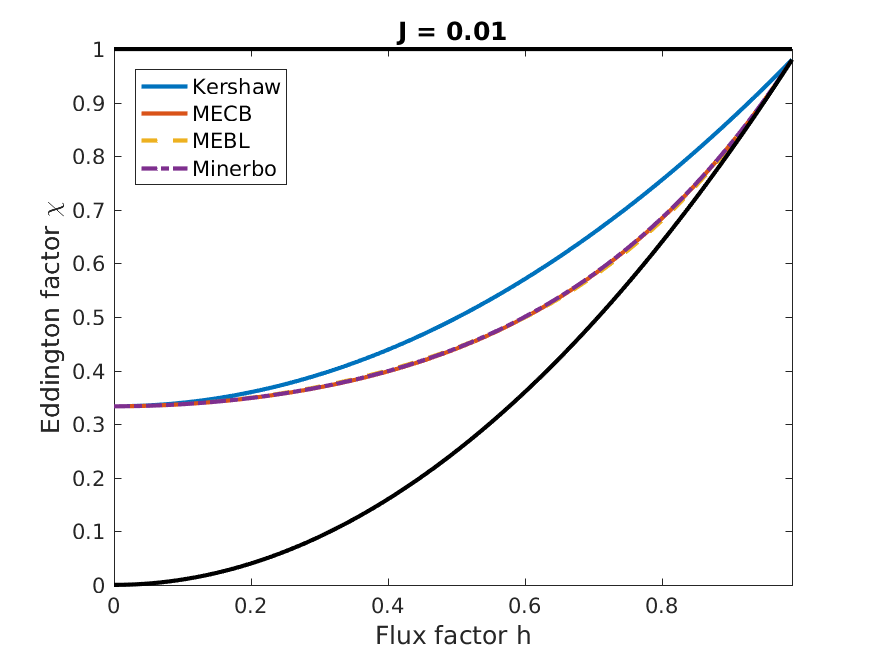
\includegraphics[width=0.5\textwidth]{figures/Closures0_01}
    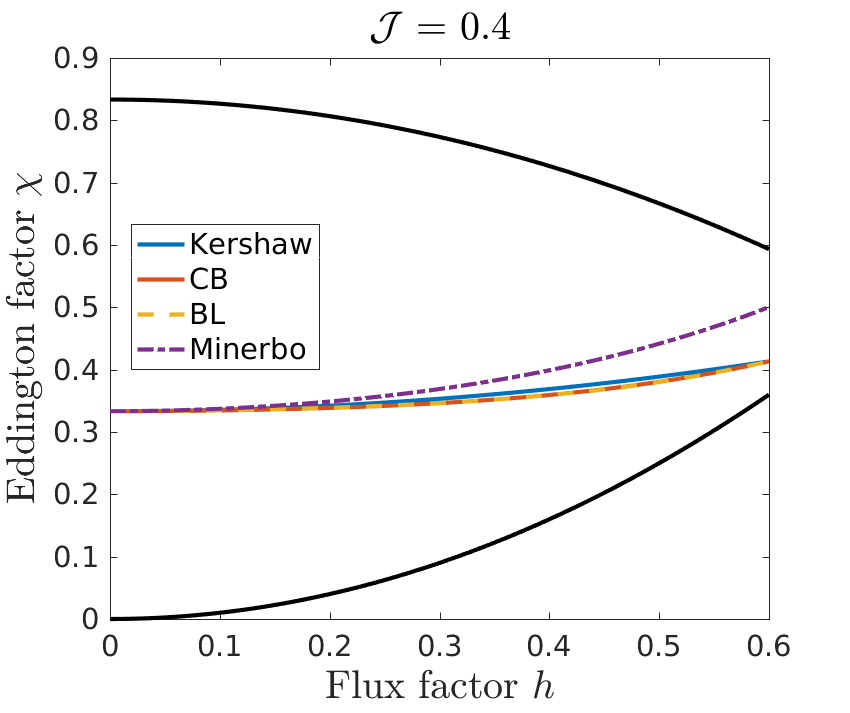
\includegraphics[width=0.5\textwidth]{figures/Closures0_40} \\
    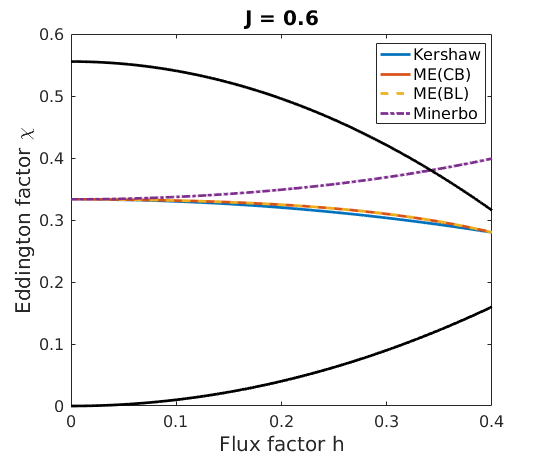
\includegraphics[width=0.5\textwidth]{figures/Closures0_60}
    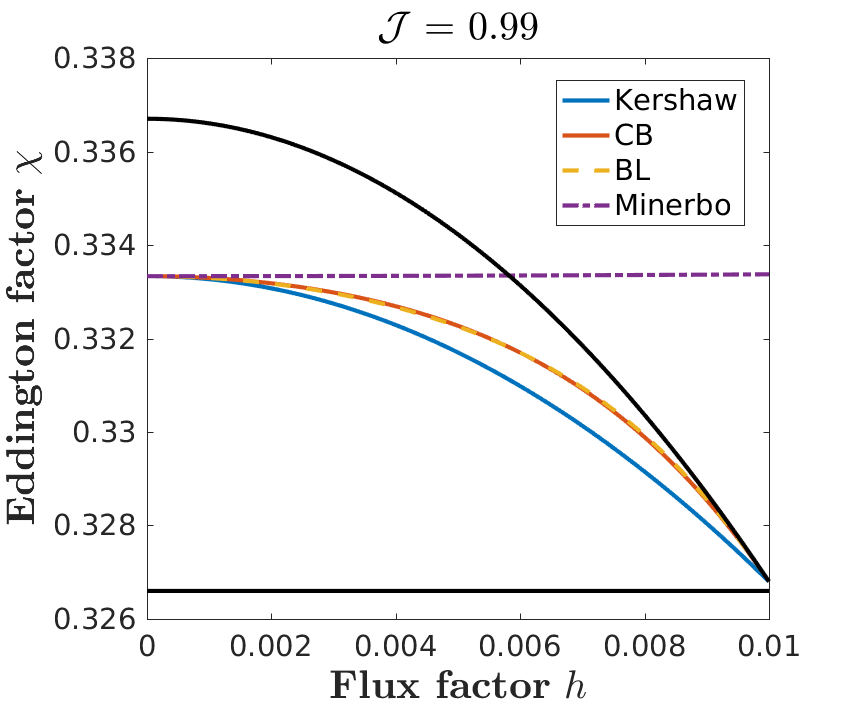
\includegraphics[width=0.5\textwidth]{figures/Closures0_99}
  \end{tabular}
   \caption{Plot of Eddington factors $\chi$ versus flux factor $h$ for different values of $\cJ$ for various algebraic closures: $\cJ=0.01$ (upper left panel), $\cJ=0.4$ (upper right panel), $\cJ=0.6$ (lower left panel), and $\cJ=0.99$ (lower right panel).  In each panel we plot the Eddington factors of Kershaw (solid blue lines), Cernohorsky \& Bludman (CB, solid red lines), Banach \& Larecki (BL, dashed orange lines), and Minerbo (dash-dot purple lines).  We also plot $\chi_{\mbox{\tiny min}}$ and $\chi_{\mbox{\tiny max}}$ (lower and upper solid black lines, respectively).}
  \label{fig:EddingtonFactorsWithDifferentClosure}
\end{figure}
We have also checked numerically that for all the algebraic closures based on Fermi-Dirac statistics (CB, BL, and Kershaw), the bounds on the Eddington factor in Eq.~\eqref{eq:eddingtonFactorBounds} holds for all $\vect{\cM}\in\cR$.  
Thus, we conclude that these closures are suited for development of realizability-preserving numerical methods for the two-moment model of fermion transport.  

In Figure~\ref{fig:MabWithDifferentClosure}, we further illustrate the properties of the algebraic closures by plotting $\vect{\cM}_{ab}$ as defined in Lemma~\ref{lem:explicitStep}.  
In each of the four panels, representing the algebraic closures discussed above, we plot $\vect{\cM}_{ab}$ constructed from randomly selected pairs $\vect{\cM}_{a},\vect{\cM}_{b}\in\cR$ (each blue dot represents one realization of $\vect{\cM}_{ab}$).  
Results for the maximum entropy closures of BL and CB are plotted in the upper panels (left and right panel, respectively).  
Results for the Kershaw closure are plotted in the lower left panel, while results for the Minerbo closure are plotted in the lower right panel.  
As expected for closures consistent with moments of a Fermi-Dirac distribution function, we find $\vect{\cM}_{ab}\in\cR$ for the CB, BL, and Kershaw closures.  
For the Minerbo closure (right bottom), which is consistent with positive distributions, $\vect{\cM}_{ab}$ is not confined to $\cR$.  
\begin{figure}[h]
  \centering
  \begin{tabular}{cc}
    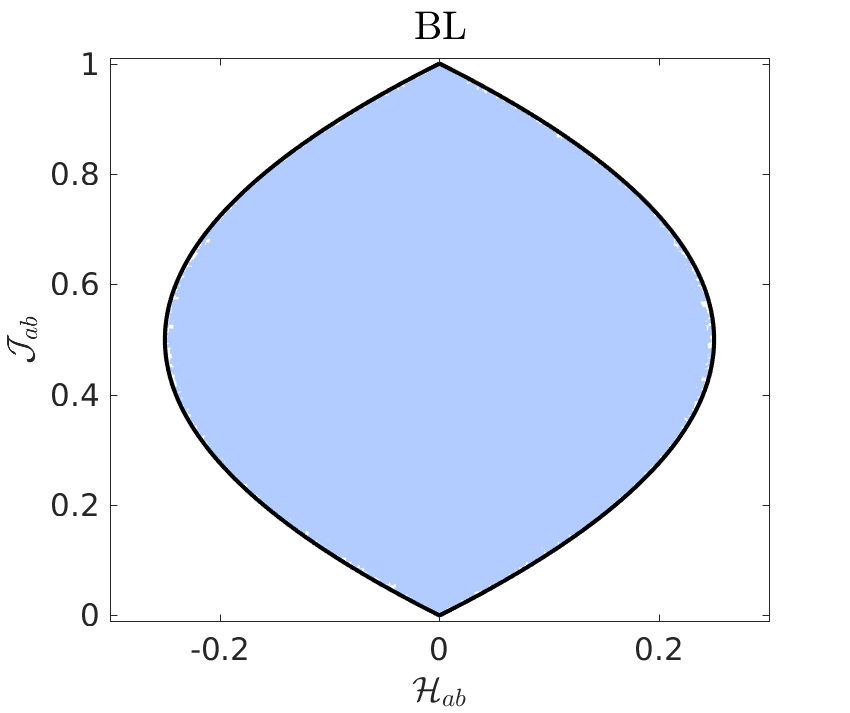
\includegraphics[width=0.5\textwidth]{figures/MabWithBLME}
    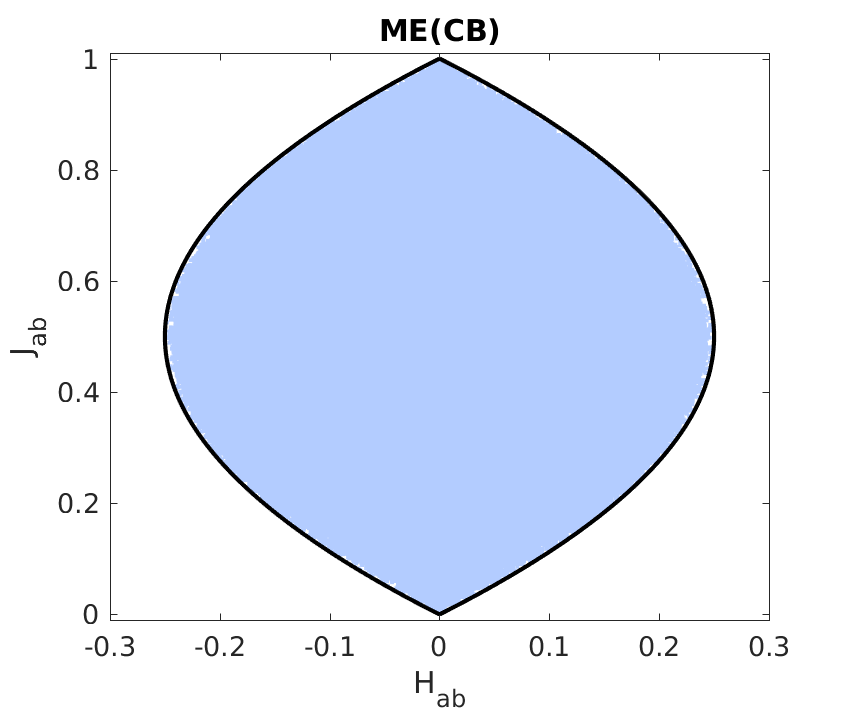
\includegraphics[width=0.5\textwidth]{figures/MabWithCBME} \\
    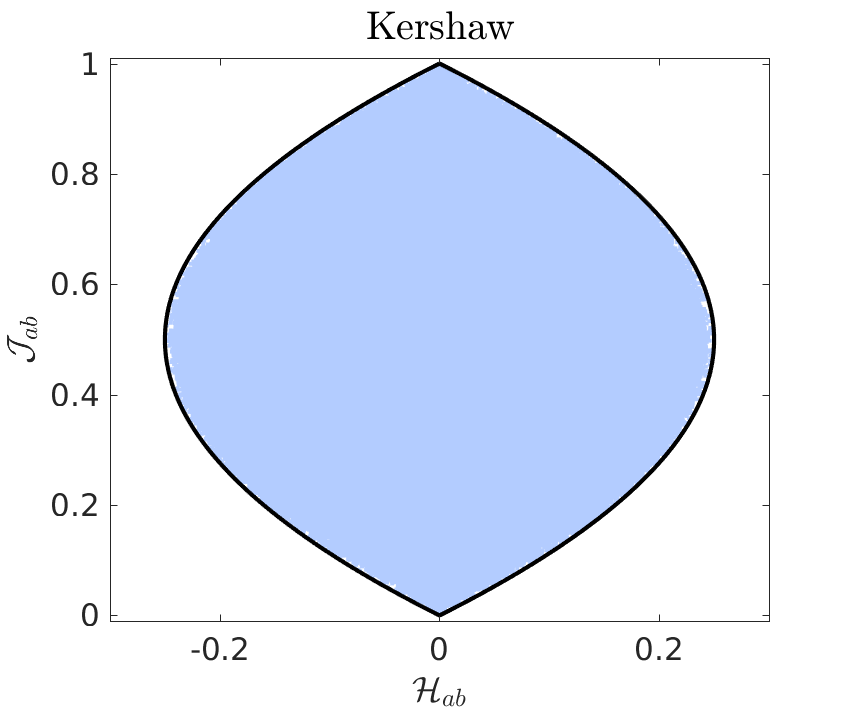
\includegraphics[width=0.5\textwidth]{figures/MabWithBLKS}
    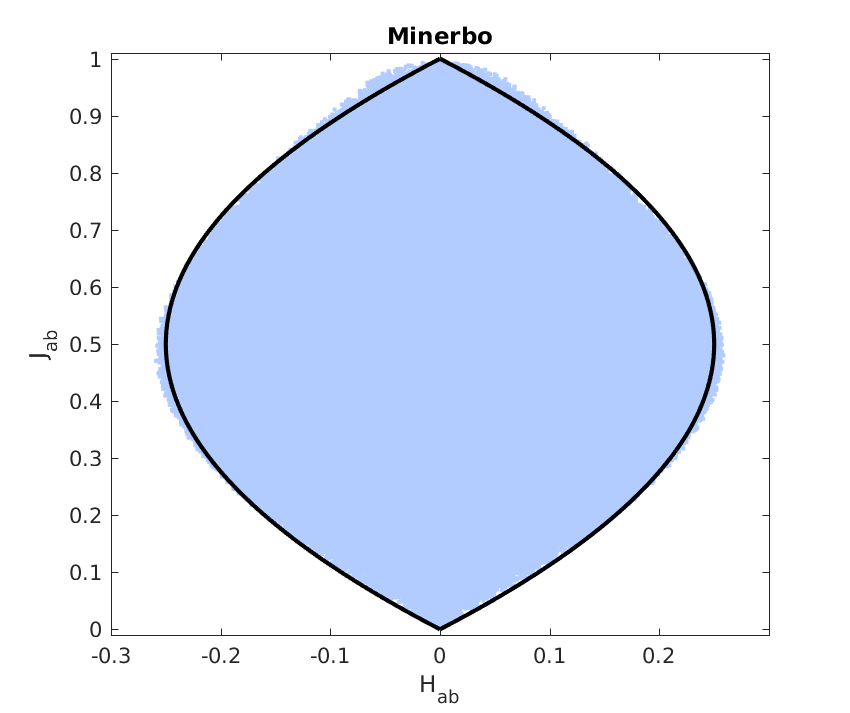
\includegraphics[width=0.5\textwidth]{figures/MabWithMI}
  \end{tabular}
   \caption{Illustration of $\vect{\cM}_{ab}$, as defined in Lemma~\ref{lem:explicitStep}, computed with different algebraic closures: the maximum entropy closures of Banach \& Larecki (top left) and Cernohorsky \& Bludman (top right), the Kershaw closure (bottom left), and the maximum entropy closure of Minerbo (bottom right).  In each panel, $\vect{\cM}_{ab}$ was computed using the respective closure, using $10^{6}$ random pairs ($\vect{\cM}_{a},\vect{\cM}_{b}\in\cR$), and plotted as a light-blue point.  The solid black lines mark the boundary of $\cR$: $\gamma(\vect{\cM}) = 0$.}
  \label{fig:MabWithDifferentClosure}
\end{figure}
\section{Discontinuous Galerkin Method}
\label{sec:dg}

Here we briefly outline the DG method for the moment equations.  
(See, e.g., \cite{cockburnShu_2001}, for a comprehensive review on the application of DG methods to solve hyperbolic conservation laws.)  
Since we do not include any physics that couples the energy dimension, the particle energy $\epsilonNu$ is simply treated as a parameter.  
For notational convenience, we will suppress explicit energy dependence of the moments.  
Employing Cartesian coordinates, we write the moment equations in $d$ spatial dimensions as
\begin{equation}
  \pd{\vect{\cM}}{t}+\sum_{i=1}^{d}\pderiv{}{x^{i}}\big(\,\vect{\cF}^{i}(\vect{\cM})\,\big)
  =\frac{1}{\tau}\,\vect{\cC}(\vect{\cM}),
  \label{eq:angularMomentsCartesian}
\end{equation}
where $x^{i}$ is the coordinate along the $i$th coordinate dimension.  
We divide the spatial domain $D$ into a disjoint union $\mathscr{T}$ of open elements $\bK$, so that $D = \cup_{\bK \in \mathscr{T}}\bK$.  
We require that each element is a $d$-dimensional box in the logical coordinates; i.e.,
\begin{equation}
  \bK=\{\,\vect{x} : x^{i} \in K^{i} := (\xL^{i},\xH^{i}),~|~i=1,\ldots,d\,\}, 
\end{equation}
with surface elements denoted $\tilde{\bK}^{i}=\times_{j\ne i}K^{j}$.  
We let $|\bK|$ denote the volume of an element
\begin{equation}
  |\bK| = \int_{\bK}d\vect{x}, \quad\text{where}\quad d\vect{x} = \prod_{i=1}^{d}dx^{i}.  
\end{equation}
We also define $\tilde{\vect{x}}^{i}$ as the coordinates orthogonal to the $i$th dimension, so that as a set $\vect{x}=\{\tilde{\vect{x}}^{i},x^{i}\}$.  
The width of an element in the $i$th dimension is $|K^{i}|=\xH^{i}-\xL^{i}$.  

We let the approximation space for the DG method, $\mathbb{V}^{k}$, be constructed from the tensor product of one-dimensional polynomials of maximal degree $k$.  
Note that functions in $\mathbb{V}^{k}$ can be discontinuous across element interfaces.  
The semi-discrete DG problem is to find $\vect{\cM}_{h}\in\mathbb{V}^{k}$ (which approximates $\vect{\cM}$ in Eq.~\eqref{eq:angularMomentsCartesian}) such that
\begin{align}
  &\pd{}{t}\int_{\bK}\vect{\cM}_{h}\,v\,d\vect{x}
  +\sum_{i=1}^{d}\int_{\tilde{\bK}^{i}}
  \big(\,
    \widehat{\bcF}^{i}(\vect{\cM}_{h})\,v\big|_{\xH^{i}}
    -\widehat{\bcF}^{i}(\vect{\cM}_{h})\,v\big|_{\xL^{i}}
  \,\big)\,d\tilde{\bx}^{i} \nonumber \\
  &\hspace{24pt}
  -\sum_{i=1}^{d}\int_{\bK}\bcF^{i}(\vect{\cM}_{h})\,\pderiv{v}{x^{i}}\,d\vect{x}
  =\f{1}{\tau}\int_{\bK}\bcC(\vect{\cM}_{h})\,v\,d\vect{x},
  \label{eq:semidiscreteDG}
\end{align}
for all $v\in\mathbb{V}^{k}$ and all $\bK\in\mathscr{T}$.  

In Eq.~\eqref{eq:semidiscreteDG}, $\widehat{\bcF}^{i}(\vect{\cM}_{h})$ is a numerical flux, approximating the flux on the surface of $\bK$ with unit normal along the $i$th coordinate direction.  
It is evaluated with a flux function $\vect{\mathscr{F}}^{i}$ using the DG approximation from both sides of the element interface; i.e.,
\begin{equation}
  \widehat{\bcF}^{i}(\vect{\cM}_{h})\big|_{x^{i}}=\vect{\mathscr{F}}^{i}(\vect{\cM}_{h}(x^{i,-},\tilde{\bx}^{i}),\vect{\cM}_{h}(x^{i,+},\tilde{\bx}^{i})),
\end{equation}
where superscripts $-/+$ in the arguments of $\vect{\cM}_{h}$ indicate that the function is evaluated to the immediate left/right of $x^{i}$.  
In this paper we use the simple Lax-Friedrichs (LF) flux given by
\begin{equation}
  \vect{\mathscr{F}}_{\mbox{\tiny LF}}^{i}(\vect{\cM}_{a},\vect{\cM}_{b})
  =\f{1}{2}\,\big(\,\bcF^{i}(\vect{\cM}_{a})+\bcF^{i}(\vect{\cM}_{b})-\alpha^{i}\,(\,\vect{\cM}_{b}-\vect{\cM}_{a}\,)\,\big),
  \label{eq:fluxFunctionLF}
\end{equation}
where $\alpha^{i}$ is the largest eigenvalue (in absolute value) of the flux Jacobian $\partial\bcF^{i}/\partial\vect{\cM}$.  
For particles propagating at the speed of light, we can simply take $\alpha^{i}=1$ (i.e., the global LF flux).  

\begin{rem}
For simplicity, in Eq.~\eqref{eq:semidiscreteDG}, we have approximated the opacities $\sigma_{\Ab}$ and $\sigma_{\Scatt}$ (and thus $\xi$ and $\tau$) on the right-hand side of Eq.~\eqref{eq:angularMomentsCartesian} with constants in each element; i.e., $\sigma_{\Ab},\sigma_{\Scatt}\in\bbV^{0}$.  
\end{rem}
\section{Positivity-Preserving IMEX Schemes}
\label{sec:imex}

In this section we summarize and discuss the class of IMEX schemes we consider for the realizability-preserving DG-IMEX method for the two-moment model developed in Section~\ref{sec:realizableDGIMEX} (see also \ref{app:butcherTables} for additional details).  
The semi-discretization of the moment equations with the DG method given by Eq.~\eqref{eq:semidiscreteDG} results in a system of ordinary differential equations (ODEs) in each element of the form
\begin{equation}
  \dot{\vect{u}}
  =\vect{\cT}(\vect{u})+\f{1}{\tau}\,\vect{\cQ}(\vect{u}),
  \label{eq:ode}
\end{equation}
where $\vect{u}$ are the degrees of freedom evolved with the DG method; i.e., for a test space spanned by $\{\phi_{i}(\vect{x})\}_{i=1}^{N}\in\bbV^{k}$, we let
\begin{equation}
  \vect{u}=\f{1}{|\bK|}\Big(\,\int_{\bK}\vect{\cM}_{h}\,\phi_{1}\,d\vect{x},\int_{\bK}\vect{\cM}_{h}\,\phi_{2}\,d\vect{x},\ldots,\int_{\bK}\vect{\cM}_{h}\,\phi_{N}\,d\vect{x}\,\Big)^{T}.
\end{equation}
Thus, for $\phi_{1}=1$, the first components of $\vect{u}$ are the cell averaged moments.  
In Eq.~\eqref{eq:ode}, the transport term $\vect{\cT}$ is due to the second and third term on the left-hand side of Eq.~\eqref{eq:semidiscreteDG}, while the collision term $\vect{\cQ}$ is due to the right-hand side of Eq.~\eqref{eq:semidiscreteDG}.  

\subsection{Second-Order Accurate, Positivity-Preserving IMEX Schemes}

In the applications of interest to us, the collision term is stiff ($\tau\ll1$) in regions of the computational domain and must be treated with implicit methods, while we can resolve the time scales induced by the transport term, which we will treat with explicit methods; i.e., we will use IMEX methods \cite{pareschiRusso_2005}.  
Furthermore, we would like to employ IMEX schemes that preserve realizability of the moments (subject only to a time step governed by the explicit transport term).  
Until recently, high-order (second or higher order temporal accuracy) positivity-preserving IMEX methods with time step restrictions solely due to the transport operator were not known.  
Chertock et al. \cite{chertock_etal_2015} presented second-order accurate IMEX schemes with a correction step.  
The correction step in \cite{chertock_etal_2015} includes the transport operator, and we have found that realizability is then subject to a time step restriction that scales as $\dt\propto1/\sqrt{\tau}$, which may become too restrictive.  
More recently, Hu et al. \cite{hu_etal_2017}, presented similar IMEX schemes for problems involving BGK-type collision operators, but with a correction step that does not include the transport operator.  
In this case, positivity is only subject to time step restrictions stemming from the transport operator, which is more attractive for our target application.  
These second-order accurate, $s$-stage IMEX schemes take the following form \cite{hu_etal_2017}
\begin{align}
  \vect{u}^{(i)}
  &=\vect{u}^{n}
  +\dt\sum_{j=1}^{i-1}\tilde{a}_{ij}\,\vect{\cT}(\vect{u}^{(j)})
  +\dt\sum_{j=1}^{i}a_{ij}\,\f{1}{\tau}\,\vect{\cQ}(\vect{u}^{(j)}),
  \quad i=1,\ldots,s, \label{imexStages} \\
  \tilde{\vect{u}}^{n+1}
  &=\vect{u}^{n}
  +\dt\sum_{i=1}^{s}\tilde{w}_{i}\,\vect{\cT}(\vect{u}^{(i)})
  +\dt\sum_{i=1}^{s}w_{i}\,\f{1}{\tau}\,\vect{\cQ}(\vect{u}^{(i)}), \label{imexIntermediate} \\
  \vect{u}^{n+1}
  &=\tilde{\vect{u}}^{n+1}-\alpha\,\dt^{2}\,\f{1}{\tau^{2}}\,\vect{\cQ}'(\vect{u}^{*})\,\vect{\cQ}(\vect{u}^{n+1}), \label{eq:imexCorrection}
\end{align}
where, as in standard IMEX schemes, $(\tilde{a}_{ij})$ and $(a_{ij})$, components of $s\times s$ matrices $\tilde{A}$ and $A$, respectively, and the vectors $\vect{w}^{T}=(\tilde{w}_{1},\ldots,\tilde{w}_{s})^{T}$ and $\vect{w}=(w_{1},\ldots,w_{s})^{T}$ must satisfy certain order conditions \cite{pareschiRusso_2005}.  
The coefficient in the correction step is positive, $\alpha>0$, and $\vect{\cQ}'$ is the Fr{\'e}chet derivative of the collision term evaluated at $\vect{u}^{*}$.  
For second-order accuracy, $\vect{\cQ}'$ can be evaluated using any of the stage values ($\vect{u}^{n}$, $\vect{u}^{(i)}$, or $\tilde{\vect{u}}^{n+1}$).  
For second-order temporal accuracy, the order conditions for the IMEX scheme in Eqs.~\eqref{imexStages}-\eqref{eq:imexCorrection} are
\begin{equation}
  \sum_{i=1}^{s}\tilde{w}_{i}=\sum_{i=1}^{s}w_{i}=1,
  \label{orderConditions1}
\end{equation}
and
\begin{equation}
  \sum_{i=1}^{s}\tilde{w}_{i}\,\tilde{c}_{i}
  =\sum_{i=1}^{s}\tilde{w}_{i}\,c_{i}
  =\sum_{i=1}^{s}w_{i}\,\tilde{c}_{i}
  =\sum_{i=1}^{s}w_{i}\,c_{i}-\alpha=\f{1}{2}, 
  \label{orderConditions2}
\end{equation}
where $\tilde{c}_{i}$ and $c_{i}$ are given in \ref{app:butcherTables}.  
For globally stiffly accurate (GSA) IMEX schemes, $\tilde{w}_{i}=\tilde{a}_{si}$ and $w_{i}=a_{si}$ for $i=1,\ldots,s$, so that $\tilde{\vect{u}}^{n+1}=\vect{u}^{(s)}$.  

To prove the positivity-preserving property of the IMEX scheme, Hu et al. \cite{hu_etal_2017} rewrite the stage values in Eq.~\eqref{imexStages} in the following form
\begin{equation}
  \vect{u}^{(i)}
  =\sum_{j=0}^{i-1}c_{ij}\Big[\,\vect{u}^{(j)}+\hat{c}_{ij}\,\dt\,\vect{\cT}(\vect{u}^{(j)})\,\Big]
  +a_{ii}\,\dt\,\f{1}{\tau}\,\vect{Q}(\vect{u}^{(i)}),\quad i=1,\ldots,s,
  \label{eq:imexStagesRewrite}
\end{equation}
where $c_{ij}$, and $\hat{c}_{ij}=\tilde{c}_{ij}/c_{ij}$ are computed from $\tilde{a}_{ij}$ and $a_{ij}$.
(In Eq.~\eqref{eq:imexStagesRewrite}, $\vect{u}^{(0)}=\vect{u}^{n}$.)  
Two types of IMEX schemes are considered: \emph{type A} and \emph{type ARS}.  
For IMEX schemes of type A, the matrix $A$ is invertible.  
For IMEX schemes of type ARS, the matrix $A$ can be written as
\[\left( 
   \begin{matrix} 
       0 & 0 \\ 
       0 & \hat{A}
   \end{matrix}
\right)\]
with $\hat{A}$ be invertible.
For $i=1,\ldots,s$, the coefficients
\begin{align*}
  c_{i0}
  =&\left\{
  \begin{array}{cl}
    1 - \sum_{j=1}^{i-1}c_{ij}  & \text{for type $A$,} \\
    1 - \sum_{j=2}^{i-1}c_{ij}  & \text{for type $ARS$;}
  \end{array}
  \right.\\
  \tilde{c}_{i0}
  =&\left\{
  \begin{array}{cl}
    0  & \text{for type $A$,} \\
   \tilde{a}_{i1} + \sum_{l=2}^{i-1}a_{il}\tilde{b}_{l1}  & \text{for type $ARS$;}
  \end{array}
  \right.\\
  c_{i1}
    =&\left\{
    \begin{array}{cl}
      \sum_{l =1}^{i-1} a_{il}b_{l1} & \text{for type $A$,} \\
      0  & \text{for type $ARS$;}
    \end{array}
    \right.\\
    \tilde{c}_{i1}
    =&\left\{
      \begin{array}{cl}
       \tilde{a}_{i1} + \sum_{l=2}^{i-1}a_{il}\tilde{b}_{l1} & \text{for type $A$,} \\
       0  & \text{for type $ARS$;}
      \end{array}
      \right.
\end{align*}
and the rest coefficients were defined as in \cite{hu_etal_2017}.
For type A schemes, the positivity-preserving property follows from requiring $a_{ii}>0$ and $c_{i0}\ge0$ for $i=1,\ldots,s$, and $c_{ij},\tilde{c}_{ij}\ge0$, for $i=2,\ldots,s$, $j=1,\ldots,s-1$.  
For type ARS schemes, the positivity follows from requiring $a_{ii}>0$ and $c_{i0},\tilde{c}_{i0}\ge0$ for $i=2,\ldots,s$, and $c_{ij},\tilde{c}_{ij}\ge0$ for $i=3,\ldots,s$, $j=2,\ldots,i-1$.  
Such coefficients were given in \cite{hu_etal_2017} for GSA schemes of type A with $s=3$ and type ARS with $s=4$.  
(It was also proven that $s=3$ and $s=4$ are the necessary number of stages needed for GSA second-order positivity-preserving IMEX schemes of type A and type ARS, respectively.)  

Importantly, the coefficients $c_{ij}$ in Eq.~\eqref{eq:imexStagesRewrite} satisfy $\sum_{j=0}^{i-1}c_{ij}=1$.  
This implies that, if the expression inside the square brackets in Eq.~\eqref{eq:imexStagesRewrite} is positive for all $i=2,\ldots,s$, $j=0,\ldots,i-1$, positivity of the entire sum on the right-hand side of Eq.~\eqref{eq:imexStagesRewrite} follows from convexity arguments.  
Thus, if the explicit update with the transport operator is positive for a time step $\dt_{\mbox{\tiny Ex}}$, the IMEX scheme is positivity preserving for a time step $\dt\le c_{\mbox{\tiny Sch}}\,\dt_{\mbox{\tiny Ex}}$, where
\begin{equation}
  c_{\mbox{\tiny Sch}}=\min_{ij}\,\f{1}{\hat{c}_{ij}}.  
  \label{eq:imexCFL}
\end{equation}
It is desirable to make $c_{\mbox{\tiny Sch}}$ as large (close to $1$) as possible.  
(Positivity of $\vect{u}^{(i)}$ also requires the implicit solve to preserve positivity.)  
In \cite{hu_etal_2017}, Hu et al. provide examples of GSA, positivity-preserving IMEX schemes of type A (see scheme PA2 in \ref{app:butcherTables}) and type ARS.  
In \ref{app:butcherTables}, we provide another example of a GSA, positivity-preserving IMEX scheme of type A (scheme PA2+), with a significantly larger $c_{\mbox{\tiny Sch}}$ (a factor of about $1.7$ larger).  

\subsection{Diffusion Accurate, Positivity-Preserving IMEX Schemes}

Unfortunately, the correction step in Eq.~\eqref{eq:imexCorrection} deteriorates the accuracy of the IMEX scheme when applied to the moment equations in the diffusion limit ($\xi=0$, $\tau\ll 1$).  
In the diffusion limit, to leading order in $\tau$, we have $\vect{\cH}\approx-\f{1}{3}\,\tau\,\nabla\cJ$, which is due to a balance between the transport term and the collision term in the equation for the particle flux $\vect{\cH}$.  
The absence of the transport operator in the correction step, destroys this balance.  
We demonstrate the inferior performance of IMEX schemes with the correction step given by Eq.~\eqref{eq:imexCorrection} in the diffusion limit in Section~\ref{sec:smoothProblems}.  
We have also implemented one of IMEX schemes in Chertock et al. \cite{chertock_etal_2015}, where the transport operator is included in the correction step, and found it to perform very well in the diffusion limit.  
However, we have not been able to prove sufficiently general realizability-preserving properties with this approach, without invoking a too severe time step restriction.  

We therefore proceed to design GSA positivity-preserving IMEX schemes, without the correction step, that perform better in the diffusion limit.  
To this end we define the vectors $\vec{\cJ}=(\cJ^{(1)},\ldots,\cJ^{(s)})^{T}$ and $\vec{\vect{\cH}}=(\vect{\cH}^{(1)},\ldots,\vect{\cH}^{(s)})^{T}$.  
In the context of IMEX schemes, the diffusion limit balance implies that the relation $A\,\vec{\vect{\cH}}=-\f{1}{3}\,\tau\,\tilde{A}\,\nabla\vec{\cJ}$ should hold to relate the stage values in Eq.~\eqref{imexStages}.  
For the final stage ($i=s$), 
\begin{equation}
  \vect{\cH}^{(s)}=-\f{1}{3}\,\tau\,\vect{e}_{s}^{T}A^{-1}\tilde{A}\vect{e}\,\nabla\cJ^{n}+\cO(\dt\,\tau),
\end{equation}
where $\vect{e}_{s}=(0,\ldots,0,1)^{T}$ and $\vect{e}=(1,\ldots,1)^{T}$.  
Thus, for $\vect{\cH}^{(s)}$ to be accurate in the diffusion limit, we require the IMEX coefficients to satisfy
\begin{equation}
  \vect{e}_{s}^{T}A^{-1}\tilde{A}\vect{e} = 1.
  \label{eq:diffusionCondition}
\end{equation}
Unfortunately, this requirement, together with the order conditions given by Eqs.~\eqref{orderConditions1} and \eqref{orderConditions2} (with $\alpha=0$), and the positivity conditions on $c_{ij}$ and $\tilde{c}_{ij}$, result in too many constraints.  
(\ee{Can we prove that it is impossible to find a second-order accurate, positivity-preserving IMEX scheme that is accurate in the diffusion limit?  Does the answer to this depend on $s$?})
(We are also concerned about increasing the number of stages, and thereby the number of implicit solves, since the implicit solve will dominate the computational cost of the IMEX scheme with more realistic collision operators.)
To reduce the number of constraints, and accommodate accuracy in the diffusion limit, we relax the requirement of overall second-order accuracy of the IMEX scheme.  
Instead, we only require the scheme to be second-order accurate in the streaming limit ($\vect{\cQ}=0$).  
This gives the order conditions
\begin{equation}
  \sum_{i=1}^{s}\tilde{w}_{i}=1
  \quad\text{and}\quad
  \sum_{i=1}^{s}\tilde{w}_{i}\,\tilde{c}_{i}=\f{1}{2}.  
  \label{eq:orderConditionsEx}
\end{equation}
We then seek to design GSA IMEX schemes with the following properties
\begin{itemize}
  \item Second-order in the streaming limit; i.e., satisfies Eq.~\eqref{eq:orderConditionsEx}.
  \item Well-behaved in the diffusion limit; i.e., satisfies Eq.~\eqref{eq:diffusionCondition}.
  \item Positivity-preserving (conditions given by \cite{hu_etal_2017}; with $c_{\mbox{\tiny Sch}}$ maximal).
  \item Few ($\le3$) implicit stages.
\end{itemize}
Fortunately, IMEX schemes satisfying these properties are easy to find, and we provide an example of type ARS with $s=3$ (two implicit solves) in \ref{app:butcherTables} (scheme PARSD).  
In the streaming limit, this scheme is identical to the optimal second-order accurate strong-stability preserving Runge-Kutta method \cite{gottlieb_etal_2001}.  
It is also very similar to the scheme given in \cite{mcclareen_2008} (see scheme PC2 in \ref{app:butcherTables}), which is also a GSA IMEX scheme of type ARS with $s=3$.  
Scheme PC2 is second-order in the streaming limit, has been demonstrated to work well in the diffusion limit \cite{mcclareen_2008,radice_etal_2013}, and satisfies the positivity conditions, but $c_{\mbox{\tiny Sch}}=0$ (our primary motivation for finding an alternative).  
In Section~\ref{sec:numerical}, we show numerically that the accuracy of scheme PARSD is practically identical to the accuracy of scheme PC2.  
\section{Realizability-Preserving DG-IMEX Scheme}
\label{sec:realizableDGIMEX}

The realizability preserving DG scheme is designed to ensure realizability of the cell averages in each element $\bK$, defined as
\begin{equation}
  \vect{\cM}_{\bK}
  =\f{1}{|\bK|}\int_{\bK}\vect{\cM}_{h}\,d\bx.  
\end{equation}
Then, with $v=1$ in Eq.~\eqref{eq:semidiscreteDG}, the stage values for the cell average in the IMEX scheme in Eq.~\eqref{eq:imexStagesRewrite} are given by
\begin{equation}
  \vect{\cM}_{\bK}^{(i)}
  =c_{i0}\,\vect{\cM}_{\bK}^{n}
  +\sum_{j=1}^{i-1}c_{ij}\,\vect{\cM}_{\bK}^{(ij)}
  +a_{ii}\,\dt\,\f{1}{\tau}\,\big(\,\vect{\eta}-\vect{\cD}\,\vect{\cM}_{\bK}^{(i)}\,\big),
  \label{eq:imexStagesCellAverage}
\end{equation}
where we have defined
\begin{equation}
  \vect{\cM}_{\bK}^{(ij)}
  =\vect{\cM}_{\bK}^{(j)}-\hat{c}_{ij}\,\dt\,\big\langle\,\nabla\cdot\vect{\cF}(\vect{\cM}_{h}^{(j)})\,\big\rangle_{\bK},
\end{equation}
and the cell average of the divergence operator is (cf. Section~\ref{sec:dg})
\begin{equation}
  \big\langle\,\nabla\cdot\vect{\cF}(\vect{\cM}_{h})\,\big\rangle_{\bK}
  =\f{1}{|\bK|}\sum_{i=1}^{d}\int_{\tilde{\bK}^{i}}
  \big(\,\widehat{\bcF}^{i}(\vect{\cM}_{h})\big|_{\xH^{i}}-\widehat{\bcF}^{i}(\vect{\cM}_{h})\big|_{\xL^{i}}\,\big)\,d\tilde{\vect{x}}^{i}.  
\end{equation}

\begin{lemma}
  Let $\vect{\cM}_{\bK}^{(i)}$ satisfy Eq.~\eqref{eq:imexStagesCellAverage}.
  Assume that $\vect{\cM}_{\bK}^{n}\in\cR$ and $\vect{\cM}_{\bK}^{(ij)}\in\cR\,\forall\,j\le i-1$.  
  Then, $\vect{\cM}_{\bK}^{(i)}\in\cR$.  
\end{lemma}
\begin{proof}
  The first two terms on the right-hand side of Eq.~\eqref{eq:imexStagesCellAverage} constitute a convex combination of elements in $\cR$; i.e.,
  \begin{equation*}
    c_{i0}\,\vect{\cM}_{\bK}^{n}+\sum_{j=1}^{i-1}c_{ij}\,\vect{\cM}_{\bK}^{(ij)}\in\cR.
  \end{equation*}
  Since $a_{ii}\,\dt/\tau>0$, it follows from Lemma~\ref{lem:implicitStep} that $\vect{\cM}_{\bK}^{(i)}\in\cR$.  
\end{proof}

We proceed to establish conditions for which $\vect{\cM}_{\bK}^{(ij)}\in\cR$.  
To this end, to simplify notation, we consider the moments
\begin{equation}
  \vect{\cM}_{\bK}^{*}
  =\vect{\cM}_{\bK}-\hat{c}\,\dt\,\big\langle\,\nabla\cdot\vect{\cF}(\vect{\cM}_{h})\,\big\rangle_{\bK},
\end{equation}
where $\vect{\cM}_{\bK}$ is the cell average of $\vect{\cM}_{h}\in\bbV^{k}$ and $\hat{c}\ge0$.  
\begin{lemma}
  Let $\{s_{i}\}_{i=1}^{d}$ be a set of positive constants satisfying $\sum_{i=1}^{d}=1$.  
  If for each $i\in\{1,\ldots,d\}$, 
  \begin{equation}
    \vect{\Gamma}^{i}\big[\vect{\cM}_{h}\big](\tilde{\vect{x}}^{i})
    :=\f{1}{|K^{i}|}
    \Big[\,\int_{K^{i}}\vect{\cM}_{h}\,dx^{i}-\f{\hat{c}\,\dt}{s_{i}}\big(\,\widehat{\bcF}^{i}(\vect{\cM}_{h})\big|_{\xH^{i}}-\widehat{\bcF}^{i}(\vect{\cM}_{h})\big|_{\xL^{i}}\,\big)\,\Big]\in\cR,
    \label{eq:realizableGamma}
  \end{equation}
  then $\vect{\cM}_{\bK}^{*}\in\cR$.  
\end{lemma}
\begin{proof}
  It is easy to show that $\vect{\cM}_{\bK}^{*}$ can be expressed as the convex combination
  \begin{equation}
    \sum_{i=1}^{d}s_{i}\,\f{1}{|\tilde{\vect{\bK}}^{i}|}\int_{\tilde{\bK}^{i}}\vect{\Gamma}^{i}\big[\vect{\cM}_{h}\big]\,d\tilde{\vect{x}}^{i}.  
    \label{eq:cellAverageInTermsOfGamma}
  \end{equation}
  The result follows immediately.  
\end{proof}
\begin{rem}
  If a quadrature rule $\tilde{\vect{Q}}^{i}:C^{0}\to\bbR$, with positive weights, and points defined by the set $\tilde{\vect{S}}^{i}$, is used to approximate the integral over $\tilde{\bK}^{i}$ in \eqref{eq:cellAverageInTermsOfGamma}, it is sufficient for \eqref{eq:realizableGamma} to hold in the quadrature points $\tilde{\vect{S}}^{i}\subset\tilde{\bK}^{i}$.  
\end{rem}

Next, we establish conditions for which \eqref{eq:realizableGamma} holds.  
To simplify the notation, we temporarily drop the dimension index $i$, setting $x^{i}=x$, $K^{i}=K$, $\vect{\Gamma}^{i}=\vect{\Gamma}$, etc.  
We let $\hat{Q}_{N}$ denote the $N$-point \emph{Gauss-Lobatto (GL)} quadrature rule on the interval $K=(x_{\Low},x_{\Hgh})$, with points
\begin{equation}
  \hat{S}=\left\{x_{\Low}=\hat{x}_{1},\cdots,\hat{x}_{N}=x_{\Hgh}\right\}, 
  \label{eq:quadraturePointsGL}
\end{equation}
and weights $\hat{w}_{q} \in (0,1]$, normalized so that $\sum_{q=1}^{N} \hat{w}_{q} = 1$.  
(The hat is used to denote the GL rule, which includes the endpoints of the interval $K$.)
This quadrature integrates polynomials in $x \in \bbR$ with degree $\le2N-3$ exactly.  
Then, if $\vect{\cM}_{h}$ is represented by such polynomials we have
\begin{equation}
  \int_{K} \bcM_{h}\,dx = \hat{Q}_{N}[\bcM_{h}] \equiv
  |K| \sum_{q=1}^{N} \hat{w}_{q}\,\hat{\bcM}_{q}
  \label{eq:quadratureRuleGL}
\end{equation}
where $\hat{\bcM}_{q} := \bcM_{h}(\hat{x}_q,\tilde{\vect{x}})$.  
In each element, $\hat{\vect{\cM}}_{1}=\vect{\cM}_{\Low}^{+}$ and $\hat{\vect{\cM}}_{N}=\vect{\cM}_{\Hgh}^{-}$.  

With the GL quadrature rule in \eqref{eq:quadratureRuleGL} (note $\hat{w}_{1}=\hat{w}_{N}$), we can write $\vect{\Gamma}$ as the convex combination
\begin{equation}
  \vect{\Gamma}\big[\bcM_{h}\big]
  =\sum_{q=2}^{N-1}\hat{w}_{q}\,\hat{\vect{\cM}}_{q}
  +2\,\hat{w}_{N}\,\Phi(\vect{\cM}_{\Low}^{-},\vect{\cM}_{\Low}^{+},\vect{\cM}_{\Hgh}^{-},\vect{\cM}_{\Hgh}^{+}),
  \label{eq:realizableGammaConvex}
\end{equation}
where we have defined
\begin{align}
  &\Phi(\vect{\cM}_{\Low}^{-},\vect{\cM}_{\Low}^{+},\vect{\cM}_{\Hgh}^{-},\vect{\cM}_{\Hgh}^{+}) \nonumber \\
  &\hspace{12pt}
  =\f{1}{2}\big(\,\vect{\cM}_{\Low}^{+}+\lambda\,\mathscr{F}(\vect{\cM}_{\Low}^{-},\vect{\cM}_{\Low}^{+})\,\big)
  +\f{1}{2}\big(\,\vect{\cM}_{\Hgh}^{-}-\lambda\,\mathscr{F}(\vect{\cM}_{\Hgh}^{-},\vect{\cM}_{\Hgh}^{+})\,\big),
\end{align}
with $\lambda=\hat{c}\,\dt/(s\,\hat{w}_{N}\,|K|)$.  
The following Lemma establishes sufficient conditions for realizability of $\vect{\Gamma}$, and hence $\vect{\cM}_{\bK}^{*}$.  
\begin{lemma}
  Assume that $\hat{\vect{\cM}}_{q}\in\cR$ for all $q=1,\ldots,N$ and all $\bK\in\mathscr{T}$.  
  Let the time step $\dt$ be chosen so that $\lambda\le1$.  
  Let the numerical flux be given by the Lax-Friedrichs flux in Eq.~\eqref{eq:fluxFunctionLF} with $\alpha=1$.  
  Then $\vect{\Gamma}[\bcM_{h}]\in\cR$.  
\end{lemma}
\begin{proof}
  In Eq.~\eqref{eq:realizableGammaConvex}, $\vect{\Gamma}[\vect{\cM}_{h}]$ is expressed as a convex combination.  
  By assumption, $\hat{\vect{\cM}}_{q}\in\cR$ ($q=2,\ldots,N-1$).  
  It remains to show $\Phi(\vect{\cM}_{\Low}^{-},\vect{\cM}_{\Low}^{+},\vect{\cM}_{\Hgh}^{-},\vect{\cM}_{\Hgh}^{+})\in\cR$.  
  Using the Lax-Friedrichs flux with $\alpha=1$, it is straightforward to show that
  \begin{align}
    &\Phi(\vect{\cM}_{\Low}^{-},\vect{\cM}_{\Low}^{+},\vect{\cM}_{\Hgh}^{-},\vect{\cM}_{\Hgh}^{+})
    =(1-\lambda)\,\f{1}{2}\,\big(\,\vect{\cM}_{\Low}^{+}+\vect{\cM}_{\Hgh}^{-}\,\big) \nonumber \\
    &\hspace{12pt}
    +\f{1}{2}\,\lambda\,\big(\,\Phi^{+}(\vect{\cM}_{\Low}^{-})+\Phi^{-}(\vect{\cM}_{\Hgh}^{-})\,\big)
    +\f{1}{2}\,\lambda\,\big(\,\Phi^{+}(\vect{\cM}_{\Low}^{+})+\Phi^{-}(\vect{\cM}_{\Hgh}^{+})\,\big),
    \label{eq:phiConvex}
  \end{align}
  where $\Phi^{\pm}(\vect{\cM})=\f{1}{2}\,\big(\vect{\cM}\pm\vect{e}\cdot\vect{\cF}(\vect{\cM})\big)$.  
  Since $\lambda\le1$, $\Phi$ is expressed as a convex combination of three terms.  
  By assumption, $\vect{\cM}_{\Low}^{-},\vect{\cM}_{\Low}^{+},\vect{\cM}_{\Hgh}^{-},\vect{\cM}_{\Hgh}^{+}\in\cR$, which immediately implies realizability of the first term on the right-hand side of Eq.~\eqref{eq:phiConvex}.  
  Realizability of the second and third terms follows by invoking Lemma~\ref{lem:explicitStep}.  
  This completes the proof.  
\end{proof}
\section{Realizability-Preserving Limiter}
\label{sec:limiter}

The bound-preserving DG-IMEX method developed in previous sections is designed to preserve realizability of the cell averaged moments, i.e., $\vect{\cM}_{\bK}\in\cR$, provided sufficiently accurate quadratures are used to integrate integrals in the DG method, specific CFL conditions are satisfied, and that the polynomial approximation $\vect{\cM}_{h}$, at time $t^{n}$, is realizable in a set of quadrature points in each element $\bK$.  
We denote this quadrature set by $S\subset\bK$.  
In the DG method, we use the limiter proposed by Zhang \& Shu \cite{zhangShu_2010a} for scalar conservation laws to enforce the bounds on the zeroth moment $\cJ$ (see also \cite{liuOsher_1996}).  
We replace the polynomial $\cJ_{h}^{n}(\vect{z})$ with the limited polynomial
\begin{equation}
  \tilde{\cJ}_{h}^{n}(\vect{z})
  =\vartheta_{1}\,\cJ_{h}^{n}(\vect{z})+(1-\vartheta_{1})\,\cJ_{\bK}^{n},
\end{equation}
where the limiter parameter $\vartheta_{1}$ is given by
\begin{equation}
  \vartheta_{1}
  =\min\Big\{\,\Big|\f{M-\cJ_{\bK}^{n}}{M_{S}-\cJ_{\bK}^{n}}\Big|,\Big|\f{m-\cJ_{\bK}^{n}}{m_{S}-\cJ_{\bK}^{n}}\Big|,1\,\Big\},
\end{equation}
with $m=0$ and $M=1$, and
\begin{equation}
  M_{S}=\max_{\vect{z}\in S}\cJ_{h}^{n}(\vect{z})
  \quad\text{and}\quad
  m_{S}=\min_{\vect{z}\in S}\cJ_{h}^{n}(\vect{z}).  
\end{equation}

In the next step, we ensure realizability of the moments by following the framework of \cite{zhangShu_2010b}, developed to ensure positivity of the pressure when solving the Euler equations of gas dynamics.  
We let $\widetilde{\vect{\cM}}_{h}^{n}=\big(\tilde{\cJ}_{h}^{n},\vect{\cH}_{h}^{n}\big)^{T}$.  
Then, if $\widetilde{\bcM}_{h}^{n}$ lies outside $\cR$ for any quadrature point $\vect{z}_{q}\in S$, i.e., $\gamma(\widetilde{\bcM}_{h}^{n})<0$, there exists an intersection point of the straight line, $\vect{s}_{q}(\xi)$, connecting $\vect{\cM}_{\bK}^{n}\in\cR$ and $\widetilde{\vect{\cM}}_{h}^{n}$ evaluated in the troubled quadrature point $\vect{z}_{q}$, denoted $\widetilde{\vect{\cM}}_{q}^{n}$, and the boundary of $\cR$.  
This line is given by the convex combination 
\begin{equation}
  \vect{s}_{q}(\xi)=\xi\,\widetilde{\vect{\cM}}_{q}^{n}+(1-\xi)\,\bcM_{\bK}^{n},
\end{equation}
where $\xi\in[0,1]$, and the intersection point $\xi_{q}$ is obtained by solving $\gamma(\bs_{q}(\xi))=0$ for $\xi$, using the bisection algorithm.  
We then replace the polynomial representation $\widetilde{\vect{\cM}}_{h}^{n}\to\widehat{\vect{\cM}}_{h}^{n}$, where
\begin{equation}
  \widehat{\vect{\cM}}_{h}^{n}(\vect{z})=\vartheta_{2}\,\widetilde{\vect{\cM}}_{h}^{n}(\vect{z})+(1-\vartheta_{2})\,\vect{\cM}_{\bK}^{n},
\end{equation}
and $\vartheta_{2}=\min_{q}\xi_{q}$ is the smallest $\xi$ obtained in the element by considering all the troubled quadrature points.  

We note that the realizability-preserving limiter is conservative; i.e., preserves the cell-average.  
\section{Numerical Tests}
\label{sec:numerical}

\subsection{Problems with Known Smooth Solutions}
\label{sec:smoothProblems}

To compare the accuracy of the IMEX schemes, we present results from smooth problems in streaming, absorption, and scattering dominated regimes in one spatial dimension.  
For all tests in this subsection, we use third order accurate spatial discretization (polynomials of degree $k=2$) and we employ the maximum entropy closure in the low occupancy limit (i.e., the Minerbo closure).  
We compare results obtained using IMEX schemes proposed here (PA2+ and PARSD) with IMEX schemes from Hu et al. \cite{hu_etal_2017} (PA2), McClarren et al. \cite{mcclarren_etal_2008} (PC2), Pareschi \& Russo \cite{pareschiRusso_2005} (SSP2332), and Cavaglieri \& Bewley \cite{cavaglieriBewley2015} (RKCB2).  
In the streaming test, we also include results obtained with second-order and third-order accurate explicit strong stability-preserving Runge-Kutta methods \cite{gottlieb_etal_2001} in the comparison (SSPRK2 and SSPRK3, respectively).  
See \ref{app:butcherTables} for further details.  
The time step is set to $\dt=0.1\times\dx$.  

When comparing the numerical results to analytic solutions, errors are computed in the $L^{1}$-error norm.  
We compare results either in the absolute error ($E_{\mbox{\tiny Abs}}^{1}$) or the relative error ($E_{\mbox{\tiny Rel}}^{1}$), defined for a scalar quantity $u_{h}$ (approximating $u$) as
\begin{equation}
  E_{\mbox{\tiny Abs}}^{1}[u_{h}](t)
  =\f{1}{|D|}\sum_{\bK\in\mathscr{T}}\int_{\bK}|u_{h}(\vect{x},t)-u(\vect{x},t)|\,d\vect{x}
  \label{eq:errorNormAbsolute}
\end{equation}
and
\begin{equation}
  E_{\mbox{\tiny Rel}}^{1}[u_{h}](t)
  =\f{1}{|D|}\sum_{\bK\in\mathscr{T}}\int_{\bK}|u_{h}(\vect{x},t)-u(\vect{x},t)|/|u(\vect{x},t)|\,d\vect{x},
  \label{eq:errorNormRelative}
\end{equation}
respectively.  
The integrals in Eqs.~\eqref{eq:errorNormAbsolute} and \eqref{eq:errorNormRelative} are computed with a $3$-point Gaussian quadrature.  

\subsubsection{Sine Wave: Streaming}

The first test involves the streaming part only, and does not include any collisions ($\sigma_{\Ab}=\sigma_{\Scatt}=0$).  
We consider a periodic domain $D=\{x:x\in[0,1]\}$, and let the initial condition be given by
\begin{equation}
  \cJ(x,t=0)=\cH_{x}(x,t=0)=0.5+0.49\times\sin\big(2\pi\,x\big).  
  \label{eq:initialConditionStreaming}
\end{equation}
We evolve until $t=10$, when the sine wave has completed 10 crossings of the computational domain.  
We vary the number of elements ($N$) from $8$ to $128$ and compute errors for various time stepping schemes.  

In Figure~\ref{fig:SineWaveStreaming}, the absolute error for the number density $E_{\mbox{\tiny Abs}}^{1}[\cJ_{h}](t=10)$ is plotted versus $N$ (see figure caption for details).  
Errors obtained with SSPRK3 are smallest and decrease as $N^{-3}$ (cf. bottom black dash-dot reference line), as expected for a scheme combining third-order accurate time stepping with third-order accurate spatial discretization.  
For all the other schemes, using second-order accurate explicit time stepping, the error decreases as $N^{-2}$.  
Among the second-order accurate methods, SSP2332 has the smallest error, followed by RKCB2.  
Errors for the remaining schemes (including SSPRK2) are indistinguishable on the plot.  
\begin{figure}[h]
  \centering
    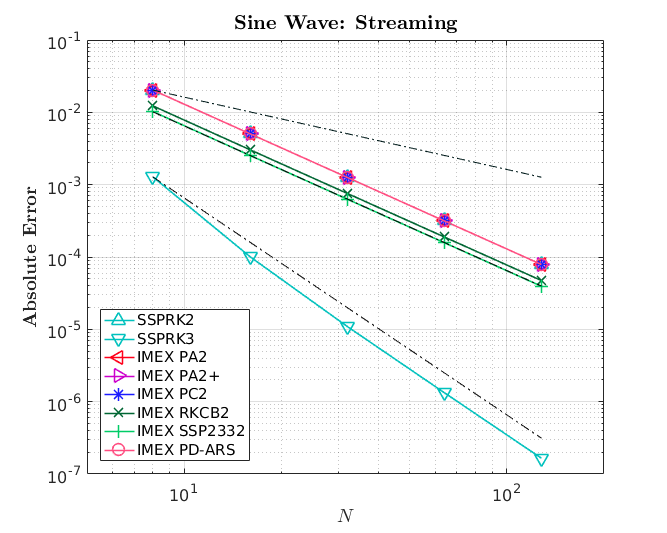
\includegraphics[width=\textwidth]{figures/SineWaveStreaming}
   \caption{Absolute error (cf. Eq.~\eqref{eq:errorNormAbsolute}) versus number of elements $N$ for the streaming sine wave test.  Results employing various time stepping schemes are compared: SSPRK2 (cyan triangles pointing up), SSPRK3 (cyan triangles pointing down), PA2 (red), PA2+ (purple), PC2 (blue), RKCB2 (dark green), SSP2332 (green), and PARSD (light red circles).  Black dash-dot reference lines are proportional to $N^{-1}$ (top), $N^{-2}$ (middle), and $N^{-3}$ (bottom), respectively.}
  \label{fig:SineWaveStreaming}
\end{figure}


\subsubsection{Sine Wave: Damping}

The next test we consider, adapted from \cite{skinnerOstriker_2013}, consists of a sine wave propagating with unit speed in a purely absorbing medium ($f_{0}=0$, $\sigma_{\Scatt}=0$), which results in exponential damping of the wave amplitude.  
We consider a periodic domain $D=\{x:x\in[0,1]\}$, and let the initial condition ($t=0$) be given as in Eq.~\eqref{eq:initialConditionStreaming}.  
For a constant absorption opacity $\sigma_{\Ab}$, the analytical solution at $t>0$ is given by
\begin{equation}
  \cJ(x,t)=\cJ_{0}(x-t)\times\exp(-\sigma_{\Ab} t)
  \quad\text{and}\quad
  \cH_{x}(x,t)=\cJ(x,t),
\end{equation}
where $\cJ_{0}(x)=\cJ(x,0)$.  

We compute numerical solutions for three values of the absorption opacity ($\sigma_{\Ab}=0.1$, $1$, and $10$), and adjust the end time $t_{\mbox{\tiny end}}$ so that $\sigma_{\Ab}t_{\mbox{\tiny end}}=10$, and the initial condition has been damped by factor $e^{-10}$.  
Thus, for $\sigma_{\Ab}=0.1$ the sine wave crosses the domain 100 times, while for $\sigma_{\Ab}=10$, it crosses the grid once.  

Figure~\ref{fig:SineWaveDamping} shows convergence results, obtained using different values of $\sigma_{\Ab}$, for various IMEX schemes at $t=t_{\mbox{\tiny end}}$.  
Results for $\sigma_{\Ab}=0.1$, $1$, and $10$ are plotted with red, green, and blue lines, respectively (see figure caption for further details).  
All the second-order accurate schemes (PA2, PA2+, RKCB2, and SSP2332) display second-order accurate convergence rates (cf. bottom, black dash-dot reference line).  
For $\sigma_{\Ab}=0.1$, SSP2332 is the most accurate among these schemes, while PA2+ is the most accurate for $\sigma_{\Ab}=10$.  
On the other hand, PC2 and PARSD are indistinguishable and display at most first-order accurate convergence, as expected.  
(For $\sigma_{\Ab}=0.1$, PC2 and PARSD are the most accurate schemes for $N=8$ and $N=16$.)

\begin{figure}[h]
  \centering
    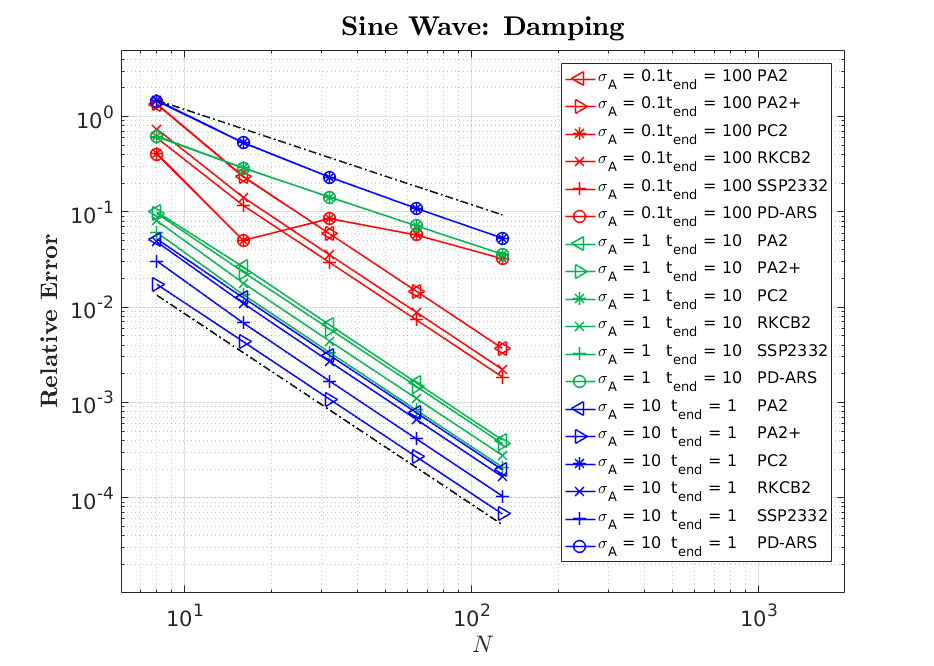
\includegraphics[width=\textwidth]{figures/SineWaveDamping}
   \caption{Relative error (cf. Eq.~\eqref{eq:errorNormRelative}) versus number of elements for the damping sine wave test.  Results for different values of the absorption opacity $\sigma_{\Ab}$, employing various IMEX time stepping schemes, are compared.  Errors for $\sigma_{\Ab}=0.1$, $1$, and $10$ are plotted with red, green, and blue lines, respectively.  The IMEX schemes employed are: PA2 (triangles pointing left), PA2+ (triangles pointing right), PC2 (asterisk), RKCB2 ($\times$), SSP2332 ($+$), and PARSD (circles).  Black dash-dot reference lines are proportional to $N^{-1}$ (top) and $N^{-2}$ (bottom), respectively.}
  \label{fig:SineWaveDamping}
\end{figure}

\subsubsection{Sine Wave: Diffusion}

The final test with known smooth solutions, adopted from \cite{radice_etal_2013}, is diffusion of a sine wave in a purely scattering medium ($f_{0}=0$, $\sigma_{\Ab}=0$).  
The computational domain $D=\{x:x\in[-3,3]\}$ is periodic, and the initial condition is given by
\begin{equation}
  \cJ_{0}(x)=0.5+0.49\times\sin\big(\pi\,x/3\big)
  \quad\text{and}\quad
  \cH_{x,0}
  =-\f{1}{3\sigma_{\Scatt}}\pderiv{\cJ_{0}}{x}.  
  \label{eq:initialConditionDiffusion}
\end{equation}
For a sufficiently high scattering opacity, the moment equations limit to a diffusion equation for the number density (deviations appear at the $1/\sigma_{\Scatt}^{2}$-level).  
With the initial conditions in Eq.~\eqref{eq:initialConditionDiffusion}, the analytical solution to the limiting diffusion equation is given by
\begin{equation}
  \cJ(x,t)=\cJ_{0}(x)\times\exp\big(-\pi^{2}\,t/(27\,\sigma_{\Scatt})\big),
\end{equation}
and $\cH_{x}=(3\,\sigma_{\Scatt})^{-1}\pd{\cJ}{x}$.  
When computing errors for this test, we compare the numerical results obtained with the two-moment model to the analytical solution to the limiting diffusion equation.  
We compute numerical solutions using three values of the scattering opacity ($\sigma_{\Scatt}=10^{2}$, $10^{3}$, and $10^{4}$), and adjust the end time so that $t_{\mbox{\tiny end}}/\sigma_{\Scatt}=1$.  
The initial amplitude of the sine wave has then been reduced by a factor $e^{-\pi^{2}/27}\approx0.694$ for all values of $\sigma_{\Scatt}$.  

\begin{figure}[h]
  \centering
  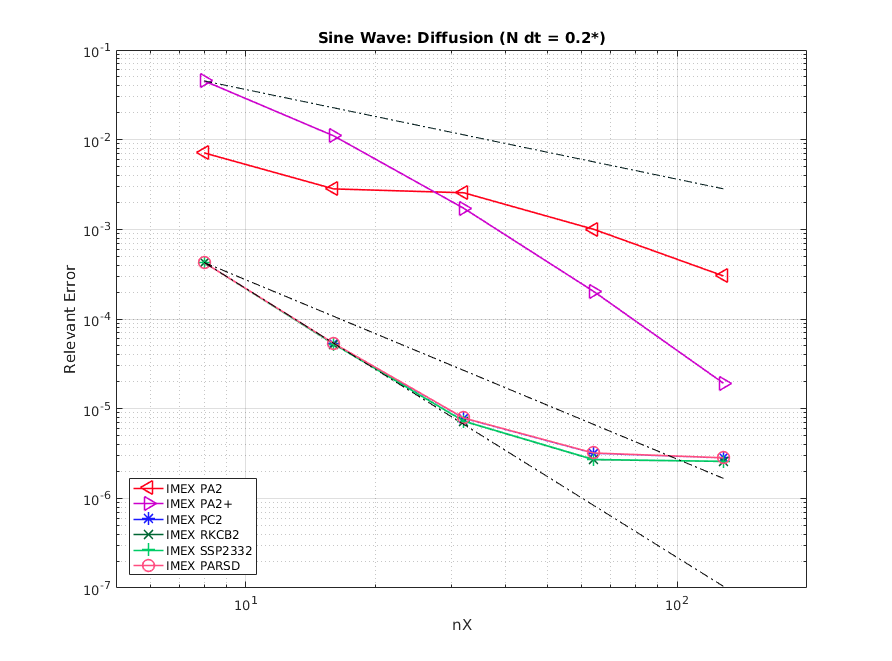
\includegraphics[width=1.0\textwidth]{figures/SineWaveDiffusionN}
   \caption{Absolute error (cf. Eq.~\eqref{eq:errorNormAbsolute}) for the number density $\cJ$ versus number of elements for the sine wave diffusion test.  Results with different values of the scattering opacity $\sigma_{\Scatt}$, employing different IMEX schemes, are compared.  Errors with $\sigma_{\Scatt}=10^{2}$, $10^{3}$, and $10^{4}$ are plotted with red, green, and blue lines, respectively.  The IMEX schemes employed are: PA2 (triangle pointing left), PA2+ (triangle pointing right), PC2 (asterisk), RKCB2 (cross), SSP2332 (plus), and PARSD (circle).  Black dash-dot reference lines are proportional to $N^{-1}$ (top) and $N^{-2}$ (bottom), respectively.}
  \label{fig:SineWaveDiffusionJ}
\end{figure}

\begin{figure}[h]
  \centering
  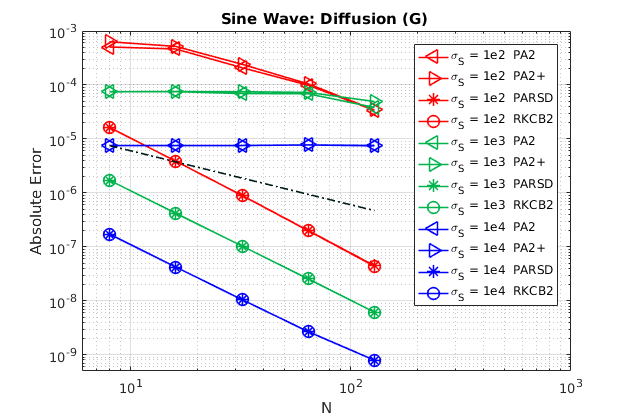
\includegraphics[width=1.0\textwidth]{figures/SineWaveDiffusionG}
   \caption{Same as in Figure~\ref{fig:SineWaveDiffusionJ}, but for the number flux $\cH_{x}$.}
  \label{fig:SineWaveDiffusionH}
\end{figure}

In Figures~\ref{fig:SineWaveDiffusionJ} and \ref{fig:SineWaveDiffusionJ} we plot the absolute error, obtained using different values of $\sigma_{\Scatt}$, for various IMEX schemes at $t=t_{\mbox{\tiny end}}$.  
Results for $\sigma_{\Scatt}=10^{2}$, $10^{3}$, and $10^{4}$ are plotted with red, green, and blue lines, respectively (see figure caption for further details).  
(Scheme PC2 has been shown to work well for this test \cite{radice_etal_2013}, but is included here for comparison with the other IMEX schemes.)
Schemes PARSD, RKCB2, and SSP2332 are accurate for this test, and display third-order accuracy for the number density $\cJ$ and second-oder accuracy for $\cH_{x}$.  
For $\sigma=10^{2}$, the errors do not drop below $10^{-6}$ because of differences between the two-moment model and the diffusion equation used to obtain the analytic solution.  
For larger values of the scattering opacity, the two-moment model agrees better with the diffusion model, and we observe convergence over the entire range of $N$.  
Schemes PA2 and PA2+ do not perform well on this test (for reasons discussed in Section~\ref{sec:imex}).  
For $\sigma_{\Scatt}=10^{2}$, errors in $\cJ$ and $\cH_{x}$ decrease with increasing $N$, but for $\sigma_{\Scatt}=10^{4}$, errors remain constant with increasing $N$ over the entire range.  

\subsection{Packed Beam}

Next we consider a one-dimensional test with discontinuous initial conditions.  
The purpose of this test is to further gauge the accuracy of the two-moment model and demonstrate the robustness of the DG scheme for dynamics close to the boundary of the realizable set $\cR$.  
The computational domain is $D=\{x:x\in[-1,1]\}$, and the initial condition is obtained from a distribution function given by
\begin{equation}
  f(x,\mu)
  =\left\{
  \begin{array}{cl}
    1        & \text{if} ~ x\le x_{\mbox{\tiny D}}, ~ \mu\ge\mu_{\mbox{\tiny D}} \\
    \delta & \text{if} ~ x\le x_{\mbox{\tiny D}}, ~ \mu<   \mu_{\mbox{\tiny D}} \\
    \delta & \text{otherwise},
  \end{array}
  \right.
\end{equation}
so that, with $\mu_{\mbox{\tiny D}}=0$, $\vect{\cM}\equiv\vect{\cM}_{\mbox{\tiny L}}=\big(0.5\,(1+\delta),0.25\,(1-\delta)\big)^{T}$ for $x\le x_{\mbox{\tiny D}}$, and $\vect{\cM}\equiv\vect{\cM}_{\mbox{\tiny R}}=\big(\delta,0\big)^{T}$ for $x> x_{\mbox{\tiny D}}$, where $\delta>0$ is a small parameter ($\delta\ll1$).  
We let $\delta=10^{-8}$, so that the initial conditions are very close to the boundary of the realizable domain (cf. Figure~\ref{fig:RealizableSetFermionic}).  
The analytical solution can be easily obtained by solving the transport equation for all angles $\mu$ (independent linear advection equations), and taking the angular moments.  
The numerical results shown in this section were obtained with the third-order scheme (polynomials of degree $k=2$ and the SSPRK3 time stepper) using $400$ elements.  
The time step is set to $\dt=0.1\times\dx$

Figure~\ref{fig:PackedBeam} shows results for various times obtained with the two-moment model.  
In the upper panels we plot the number density, while the number flux density is plotted in the lower panels.  
Numerical solutions are plotted with solid lines, while the analytical solution is plotted with dashed lines.  
In the left panels, the algebraic maximum entropy closure of Cernohorsky \& Bludman (CB) \cite{cernohorskyBludman_1994} (cf. Eqs.~\eqref{eq:eddingtonFactor} and \eqref{eq:closureMECB}) was used, while in the right panels the Minerbo closure (cf. Eqs.~\eqref{eq:eddingtonFactorLow} and \eqref{eq:closureMECB}) was used.  
For this test, the use of the realizability-preserving limiter described in Section~\ref{sec:limiter} was essential in order to avoid numerical problems.  
For the results obtained with the CB closure, the limiter was enacted whenever moments ventured outside the realizable set given by Eq.~\eqref{eq:realizableSet}.  
For the results obtained with the Minerbo closure, which is not based on Fermi-Dirac statistics, we used a modified limiter, which was enacted when the moments ventured outside the realizable domain of positive distributions; i.e., not bounded by $f\le1$, so that $\cJ\ge0$ and $\cJ\ge|\vect{\cH}|$ (e.g., \cite{levermore_1984}; see dashed red line in Figure~\ref{fig:RealizableSetFermionic}).  

\begin{figure}[h]
  \centering
  \begin{tabular}{cc}
    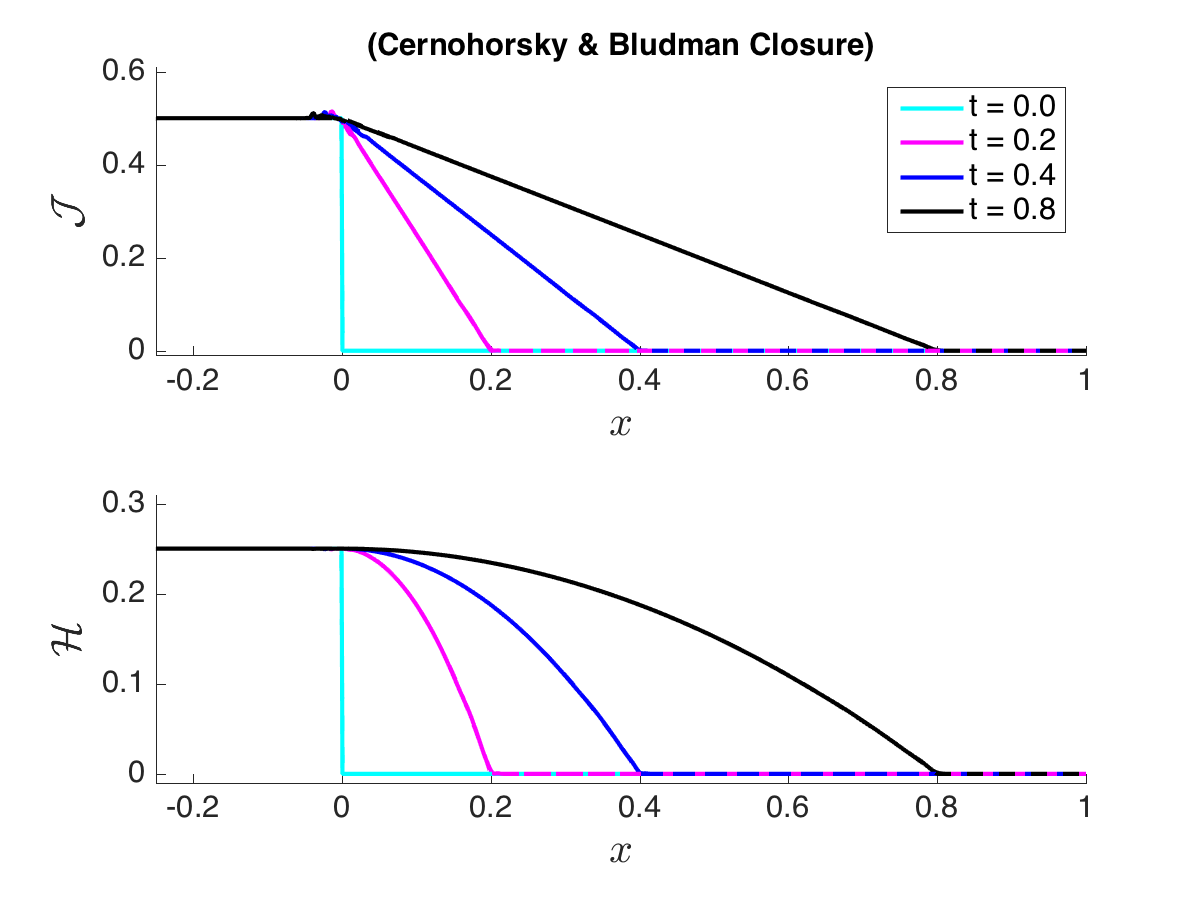
\includegraphics[width=0.485\textwidth]{figures/PackedBeam_ME_CB} &
    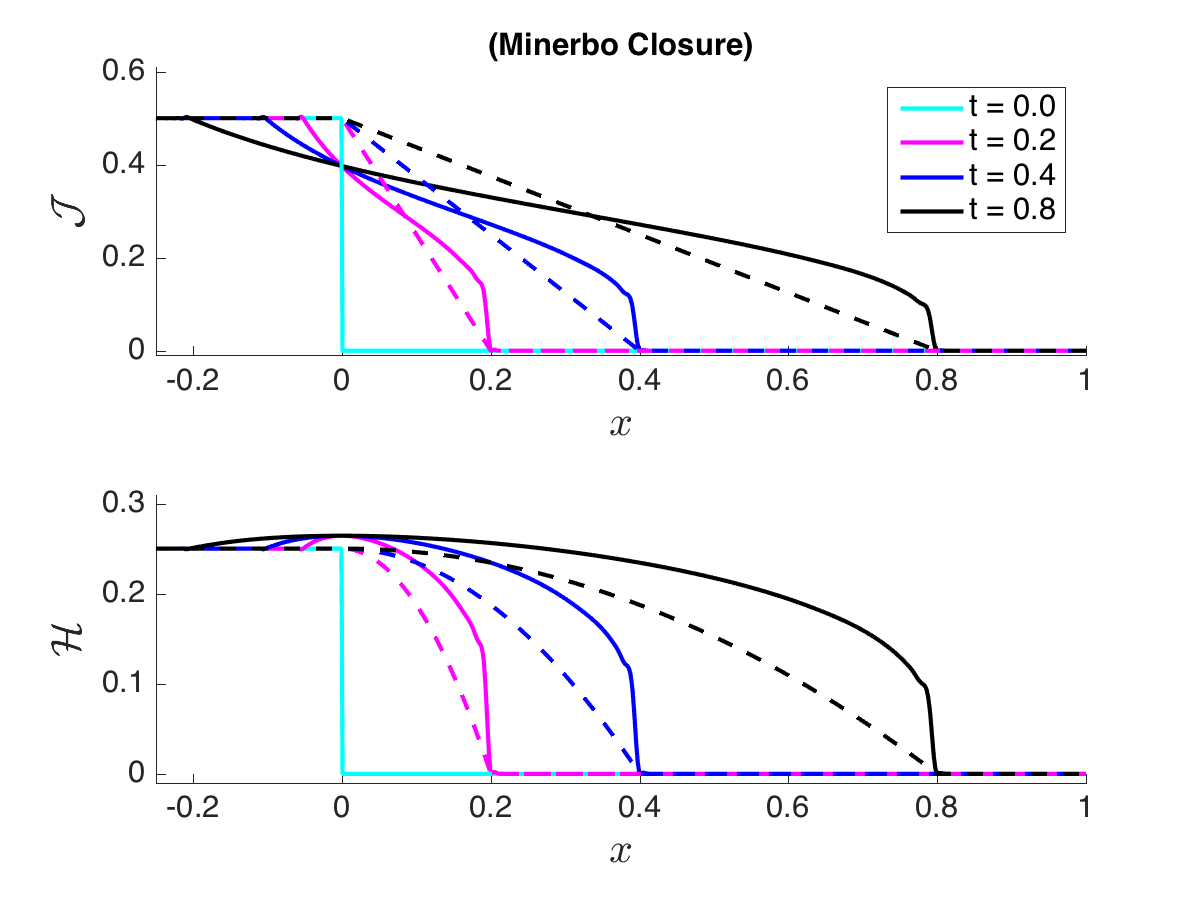
\includegraphics[width=0.485\textwidth]{figures/PackedBeam_ME_MI}
  \end{tabular}
   \caption{Numerical results from the packed beam problem at various times: $t=0$ (cyan), $t=0.2$ (magenta), $t=0.4$ (blue), and $t=0.8$ (black).  Results obtained with the Cernohorsky \& Bludman closure are displayed in the left panels, while results obtained with the Minerbo closure are displayed in the right panels.  The analytical solution (dashed lines) is also plotted.}
  \label{fig:PackedBeam}
\end{figure}

As can be seen in Figure~\ref{fig:PackedBeam}, with the CB closure the numerical solution obtained with the two-moment model tracks the analytic solution well, while with the Minerbo closure the numerical solution deviates substantially from the analytic solution.  
With the Minerbo closure, the solution also evolves outside the realizable domain for Fermi-Dirac statistics.  

In the left panel in Figure~\ref{fig:PackedBeam_Realizability} we plot $\gamma(\vect{\cM})=\big(1-\cJ\big)\,\cJ-|\vect{\cH}|$ versus position for various times.  
With the Minerbo closure, $\gamma(\vect{\cM})$ becomes negative in regions of the computational domain (dashed lines), while $\gamma(\vect{\cM})$ remains positive for all $x$ and $t$ the CB closure.  
In the right panel of Figure~\ref{fig:PackedBeam_Realizability} we plot the numerical solutions in the $(\cH,\cJ)$-plane.  
Initially, the moments are located in two points: $\vect{\cM}_{\mbox{\tiny L}}$ and $\vect{\cM}_{\mbox{\tiny R}}$, for $x\le0$ and $x>0$, respectively.  
For $t>0$, the solutions trace out curves in the $(\cH,\cJ)$-plane, connecting $\vect{\cM}_{\mbox{\tiny L}}$ and $\vect{\cM}_{\mbox{\tiny R}}$.  
With the CB closure, the solution curve (blue points) follows the boundary of the realizable set $\cR$ defined in Eq.~\eqref{eq:realizableSet} (cf. black line in Figure~\ref{fig:PackedBeam_Realizability}).  
With the Minerbo closure (magenta points), the solution follows a different curve --- outside the realizable domain for distribution functions bounded by $f\in[0,1]$, but inside the realizable domain of positive distributions (cf. red line in Figure~\ref{fig:PackedBeam_Realizability}).  
We have also run this test using the algebraic maximum entropy closure of Larecki \& Banach \cite{lareckiBanach_2011} and the simpler Kershaw-type closure in \cite{banachLarecki_2017a}.  
The numerical solutions obtained with both of these closures follow the analytic solution well, and remain within the realizable set $\cR$.  
We point out that simply using the realizability-preserving limiter described in Section~\ref{sec:limiter} with the Minerbo closure does not result in a realizability-preserving scheme for Fermi-Dirac statistics because of the properties of this closure discussed in Section~\ref{sec:algebraicClosure}, and plotted in the lower right panel of Figure~\ref{fig:MabWithDifferentClosure}.  

\begin{figure}[h]
  \centering
  \begin{tabular}{cc}
    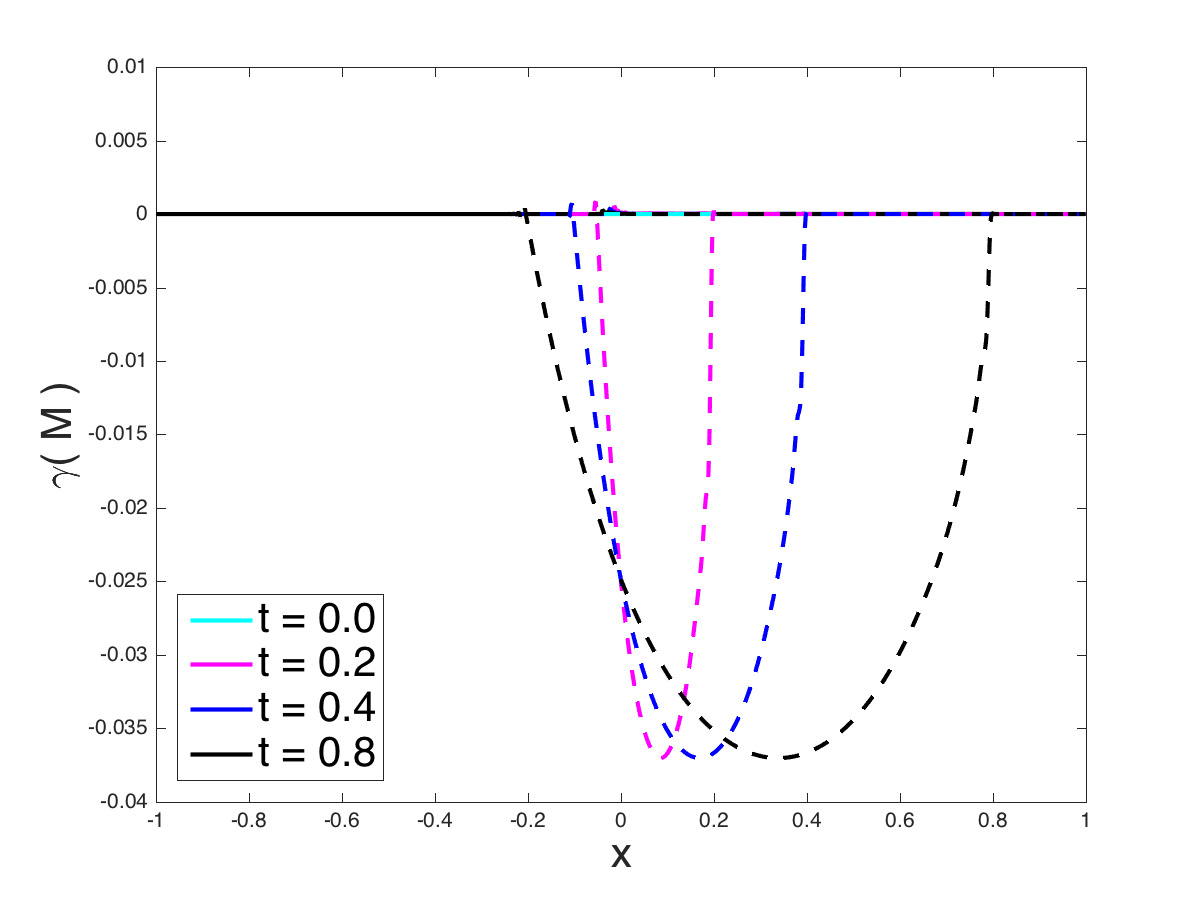
\includegraphics[width=0.485\textwidth]{figures/PackedBeam_Realizability} &
    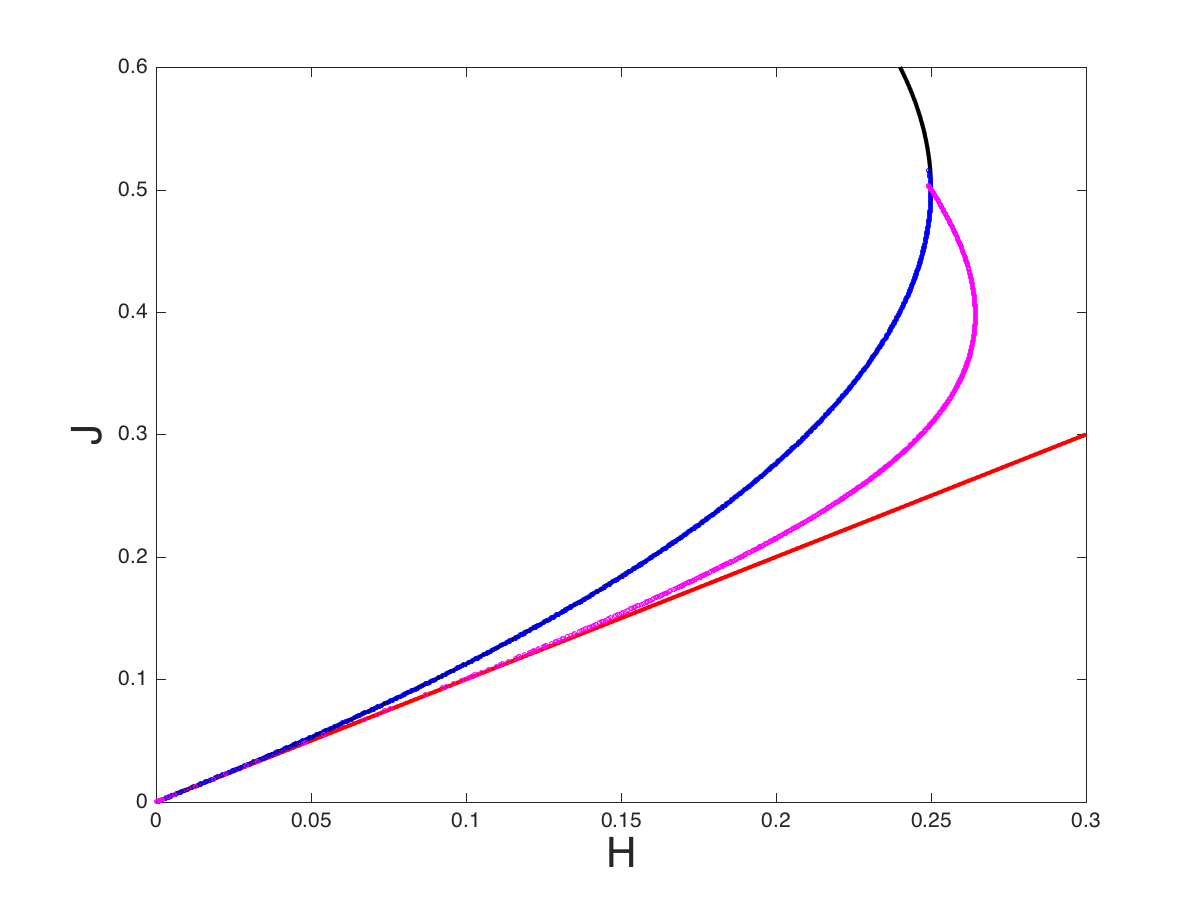
\includegraphics[width=0.485\textwidth]{figures/PackedBeam_RealizableDomain}
  \end{tabular}
   \caption{In the left panel, $\gamma(\vect{\cM})=(1-\cJ)\,\cJ-|\vect{\cH}|$ is plotted versus $x$ for various times in the packed beam problem: $t=0$ (cyan), $t=0.2$ (magenta), $t=0.4$ (blue), and $t=0.8$ (black).  Results obtained with the CB closure, which remain positive throughout the evolution, are plotted with solid lines, while results obtained with the Minerbo closure are plotted with dashed lines.  In the right panel, the moments are plotted in the $(\cH,\cJ)$-plane for the same times as in the left panel.  Results obtained with the CB and Minerbo closures are plotted in blue and magenta, respectively.  The solid black and red lines are contours where $(1-\cJ)\,\cJ=\cH$ and $\cJ=\cH$, respectively.}
  \label{fig:PackedBeam_Realizability}
\end{figure}

\subsection{Fermion Implosion}

The next test is inspired by line source benchmark (cf. \cite{brunner_2002,garrettHauck_2013}), which is a challenging test for approximate transport algorithms.  
The original line source test consists of an initial delta function particle distribution in radius $R=|\vect{x}|$; i.e., $f_{0}=\delta(R)/4\,\pi$.  
For $t>0$, a radiation front propagates in the radial direction, away from the initial source.  
Apart from capturing details of the exact transport solution, maintaining realizability of the two-moment solution is challenging.  

Here, a modified version of the line source --- dubbed \emph{Fermion Implosion},  designed to test the realizability-preserving properties of the two moment model for fermionic transport --- is computed on a two-dimensional domain with $D=\{\vect{x}\in\bbR^{2}:x^{1}\in[-1.28,1.28], x^{2}\in[-1.28,1.28]\}$.  
Instead of initializing with a delta function, we follow the initialization procedure in \cite{garrettHauck_2013}, and approximate the initial condition with an isotropic Gaussian distribution function.  
Morover, the initial distribution function is bounded $f_{\mbox{\tiny G},0}\in(0,1)$ and reaches a minimum in the center of the computational domain (hence implosion)
\begin{equation}
  f_{\mbox{\tiny G},0}
  =1-\max\Big[\,e^{-R^{2}/(2\,\sigma_{\mbox{\tiny G}}^{2})},10^{-8}\,\Big].  
\end{equation}
We set $\sigma_{\mbox{\tiny G}}=0.03$, and run this test to a final time of $t=1.0$.  
We run this test using a grid of $512^{2}$ elements, polynomials of degree $k=1$, and the SSPRK2 time stepping scheme; a second-order accurate scheme.  
(There are no collisions in this test; i.e., $\sigma_{\Ab}=\sigma_{\Scatt}=0$.)  
We present results using both the algebraic closure of Cernohorsky \& Bludman and the Minerbo closure.  

\begin{figure}[h]
  \centering
  \begin{tabular}{cc}
    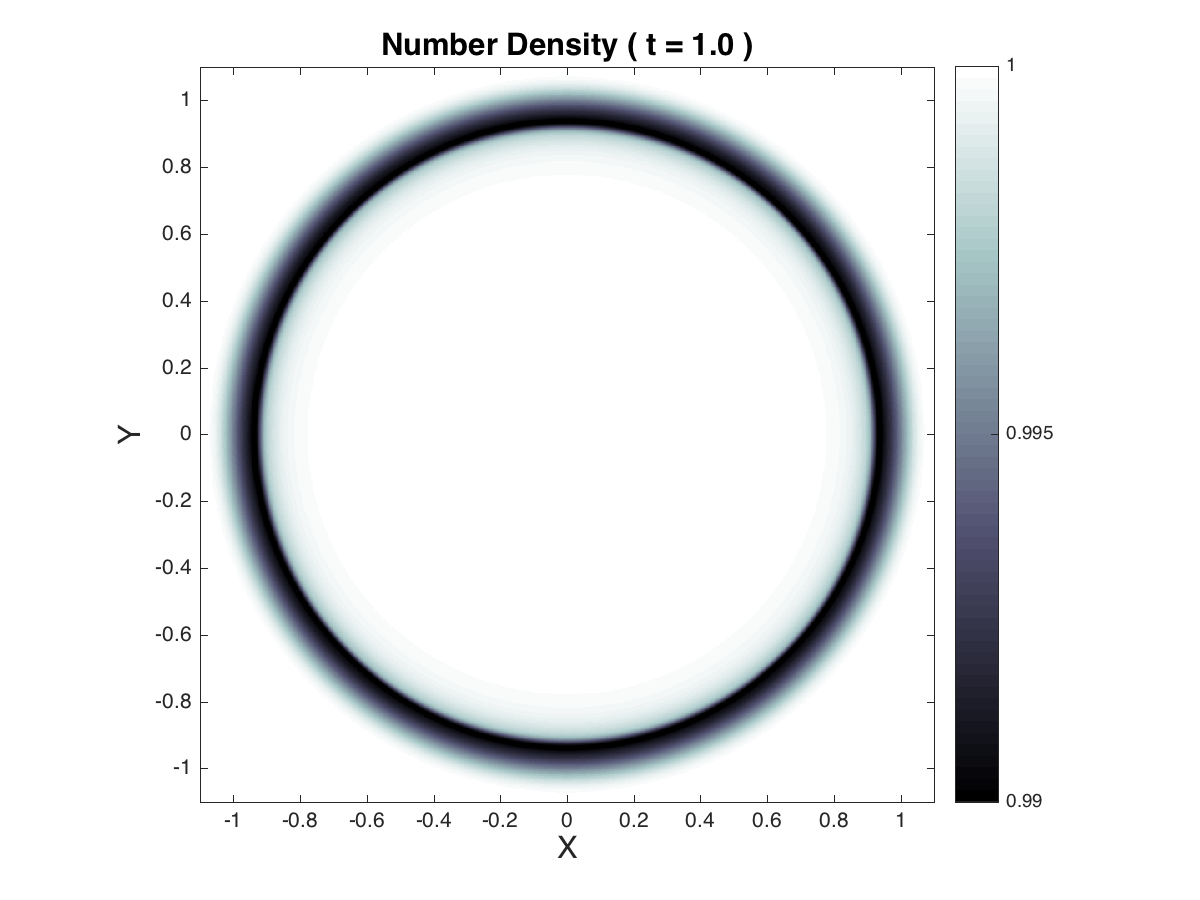
\includegraphics[width=0.495\textwidth]{figures/Implosion_Image} &
    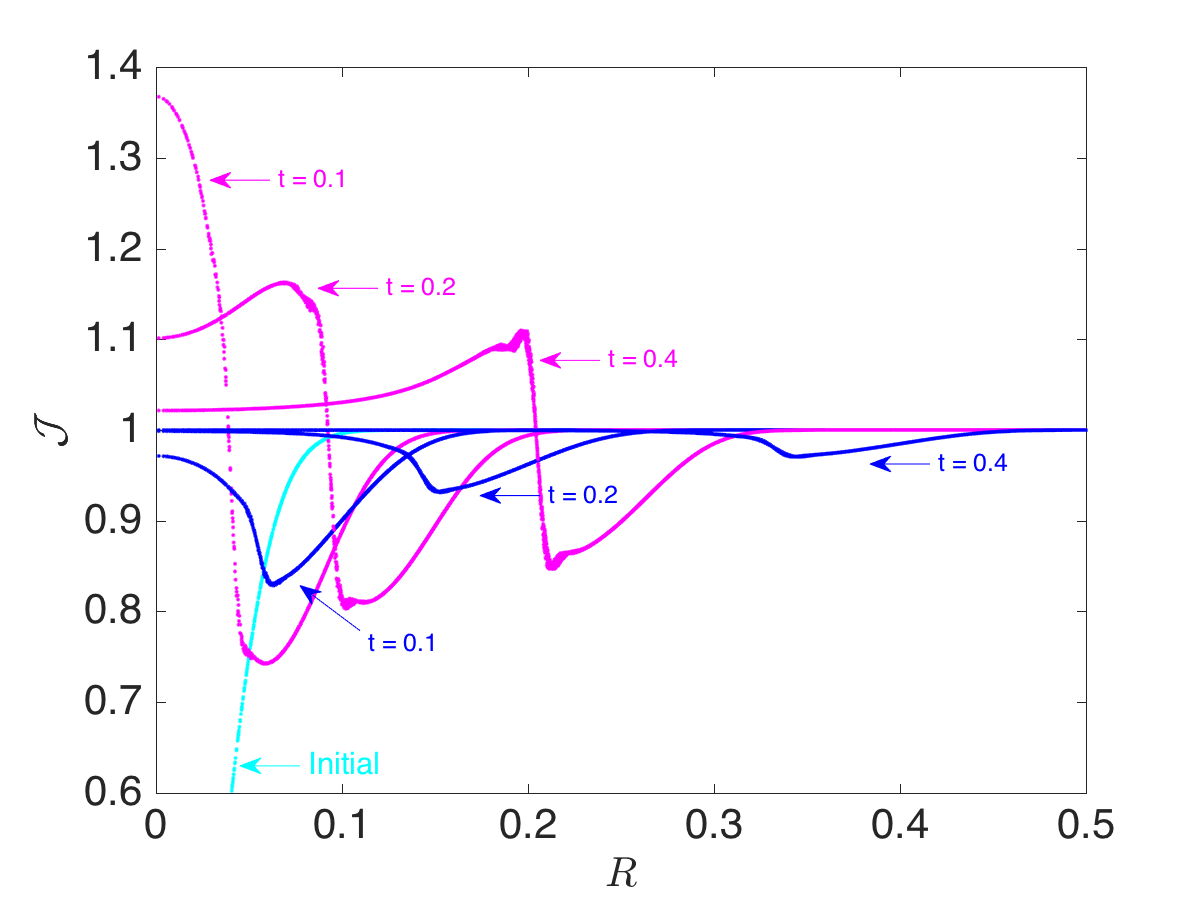
\includegraphics[width=0.495\textwidth]{figures/Implosion_Lineout} \\
    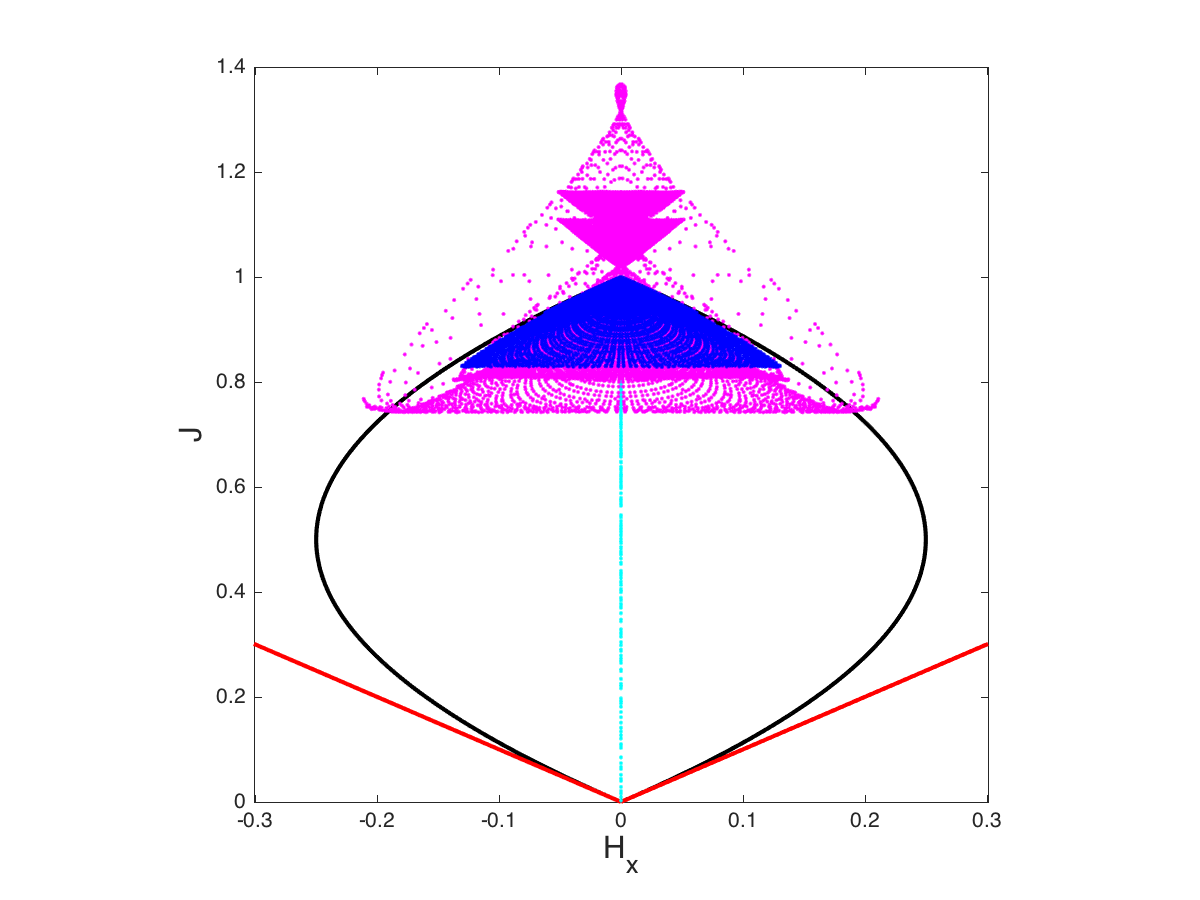
\includegraphics[width=0.495\textwidth]{figures/Implosion_RealizableDomain} &
    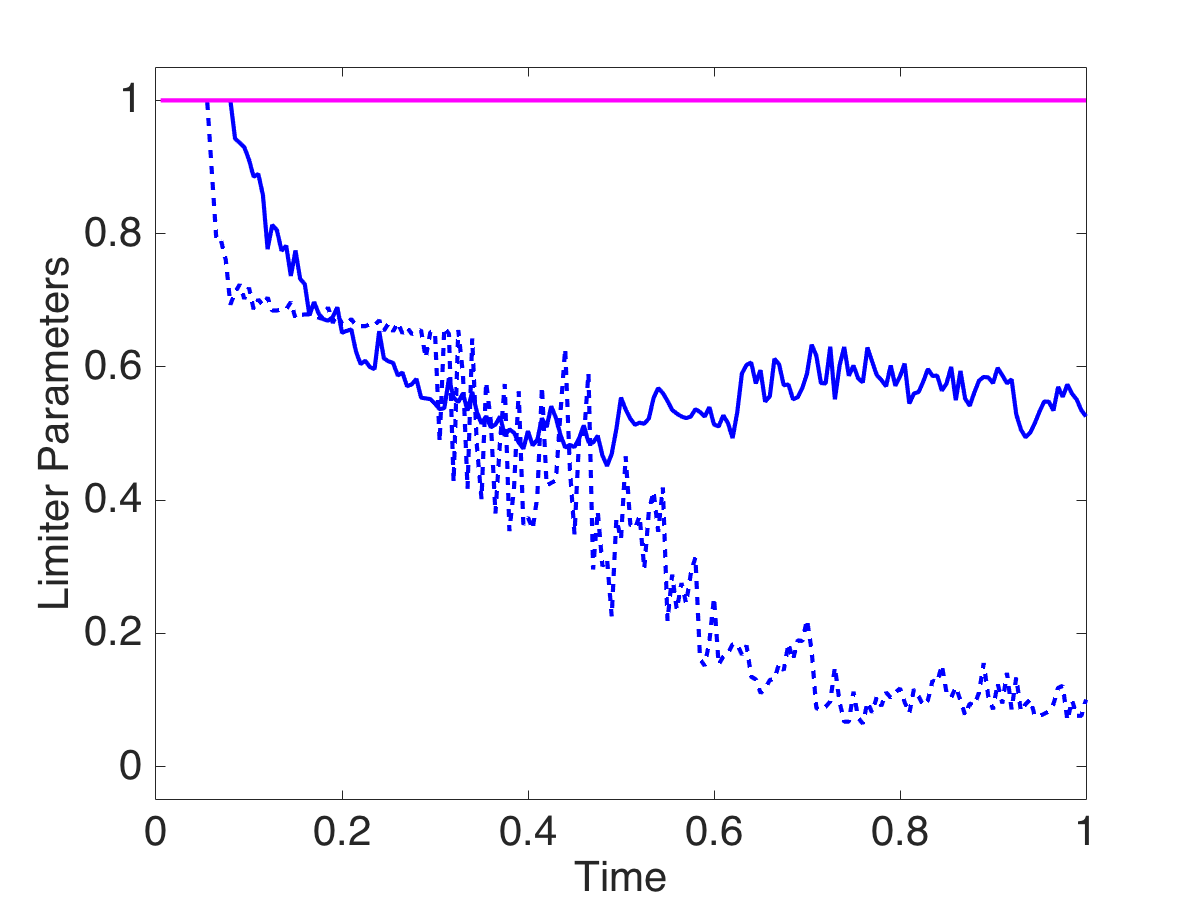
\includegraphics[width=0.495\textwidth]{figures/Implosion_LimiterParameters}
  \end{tabular}
   \caption{}
  \label{fig:Implosion}
\end{figure}

\subsection{Homogeneous Sphere}

The homogeneous sphere test (e.g., \cite{smit_etal_1997}) considers of a sphere with radius $R$.  
Inside the sphere (radius $<R$), the absorption opacity $\sigma_{\Ab}$ and the equilibrium distribution function $f_{0}$ are set to constant values.  
The scattering opacity $\sigma_{\Scatt}$ is set to zero in this test (i.e., $\xi=1$).  
Outside the sphere, the absorption opacity is zero.  
The steady state solution, obtained by solving the transport equation in spherical symmetry, is given by
\begin{equation}
  f_{\mbox{\tiny A}}(r,\mu)=f_{0}\,\big(1-e^{-\chi_{0}\,s(r,\mu)}\big),
  \label{eq:distributionHomogeneousSphere}
\end{equation}
where
\begin{equation}
  s(r,\mu)
  =\left\{
  \begin{array}{lll}
    r\,\mu+R\,g(r,\mu) & \mbox{if}\quad r<R, & \mu\in[-1,+1], \\
    2\,R\,g(r,\mu) & \mbox{if}\quad r \ge R, & \mu\in[(1-(R/r)^{2})^{1/2},+1], \\
    0 & \mbox{otherwise},
  \end{array}
  \right.
\end{equation}
and $g(r,\mu)=[1-(r/R)^{2}(1-\mu^{2})]^{1/2}$.  

\begin{figure}[h]
  \centering
  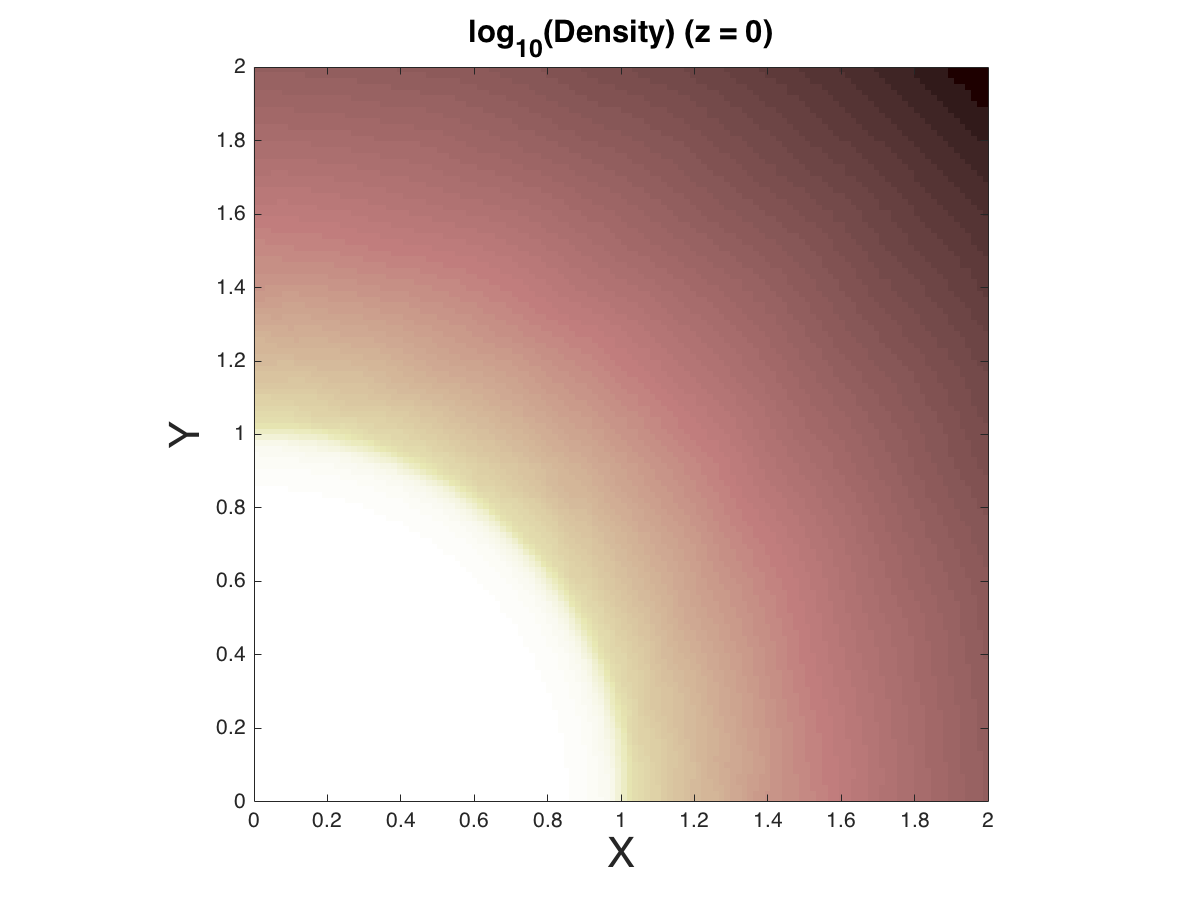
\includegraphics[width=1.0\textwidth]{figures/HomogeneousSphere_Resolution_3}
  \begin{tabular}{cc}
    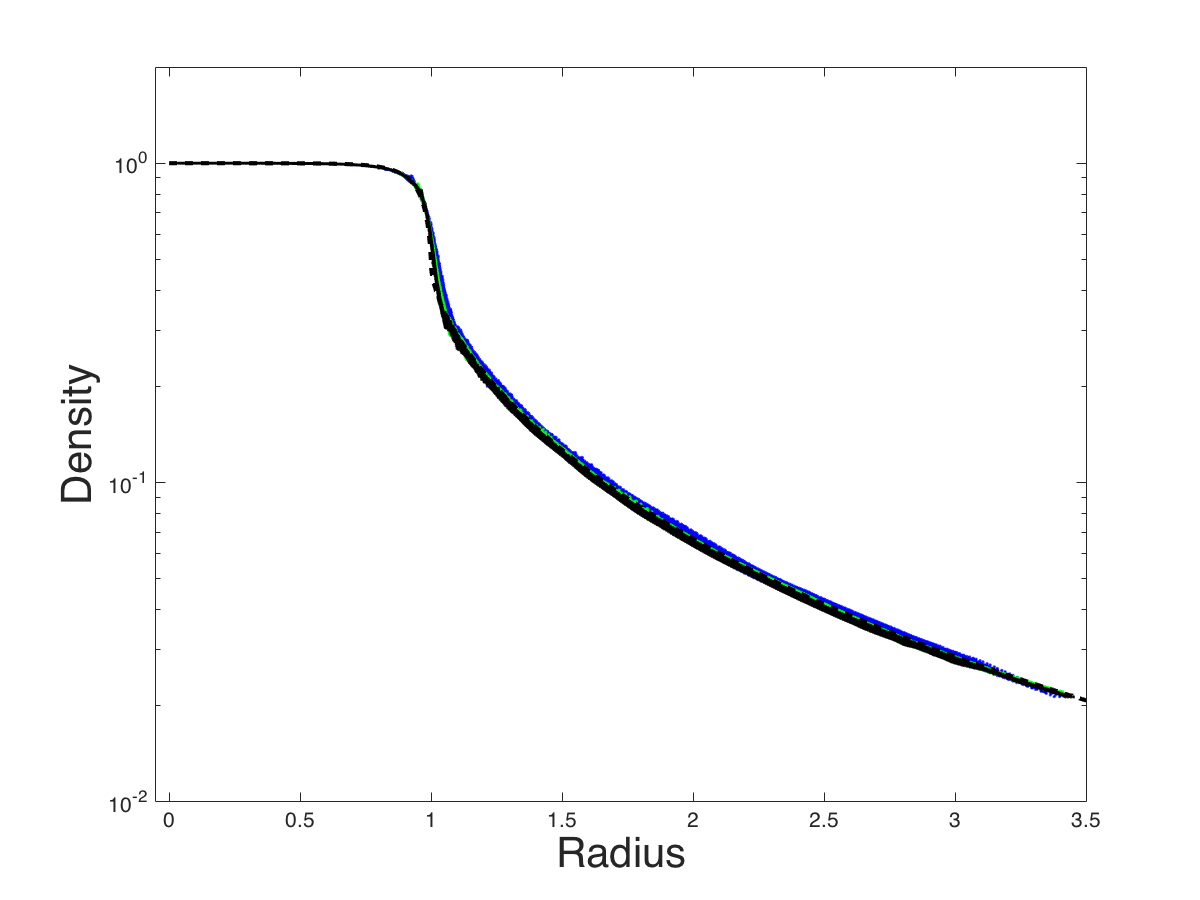
\includegraphics[width=0.5\textwidth]{figures/HomogeneousSphere_Resolution_1}
    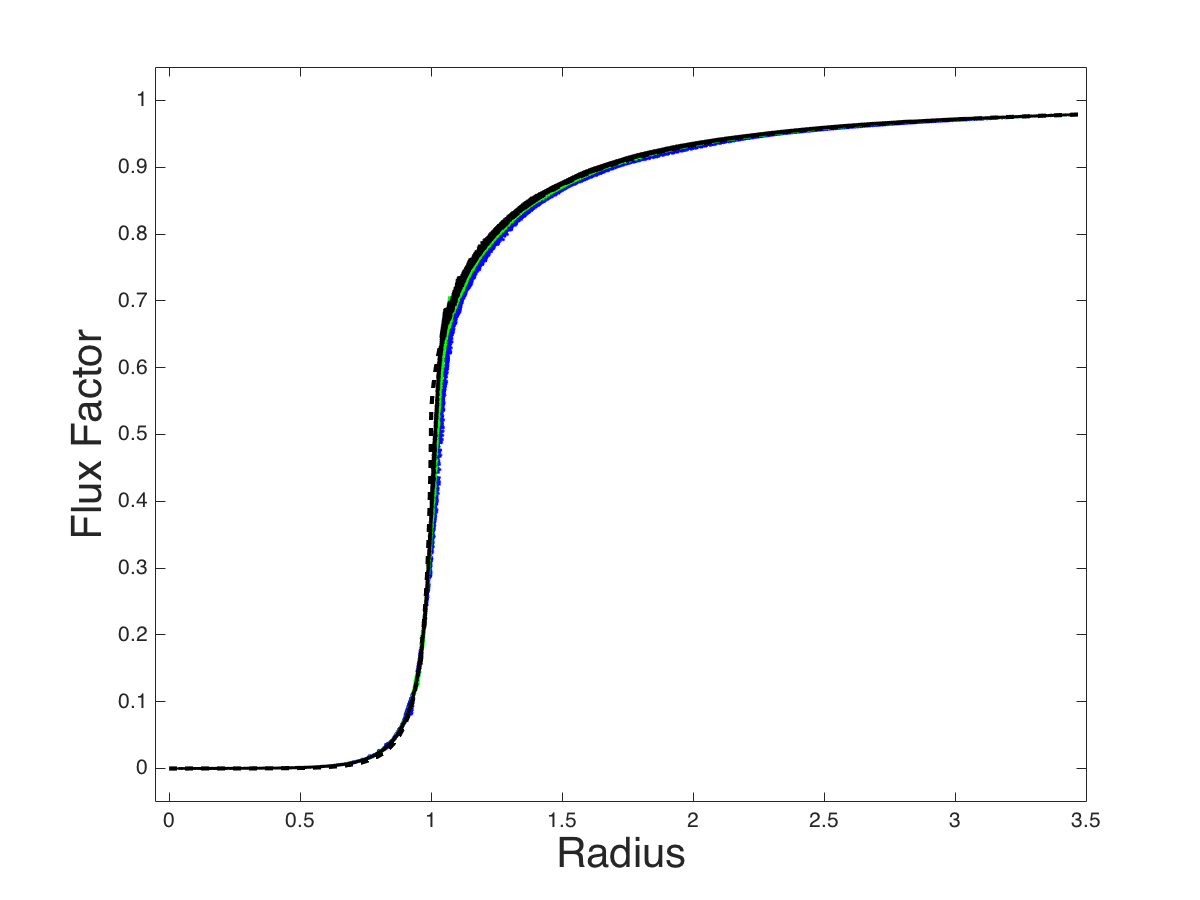
\includegraphics[width=0.5\textwidth]{figures/HomogeneousSphere_Resolution_2}
  \end{tabular}
   \caption{Homogeneous sphere problem: 32$^{3}$, 48$^{3}$, and 64$^{3}$}
  \label{fig:HomogeneousSphere_Resolution}
\end{figure}
\section{Summary and Conclusions}
\label{sec:conclusions}

We have developed a realizability-preserving DG-IMEX scheme for a two-moment model for fermion transport.  
The scheme employs simple algebraic two-moment closures rooted in Fermi-Dirac statistics, and combines a time step restriction (CFL condition), a realizability-enforcing limiter, and a constraint-preserving time integrator to maintain point-wise realizability of the moments.  
Since the realizable domain is a convex set, the realizability-preserving property is obtained from convexity arguments, building on the framework in \cite{zhangShu_2010a}.  

In the applications motivating this work, the collision term is stiff in regions of the computational domain, and we have considered IMEX schemes to avoid solving the transport operator implicitly.  
We considered recently proposed second-order accurate, constraint-preserving IMEX schemes (cf. \cite{chertock_etal_2015,hu_etal_2018}), which restore second-order accuracy with an implicit correction step.  
However, we are unable to prove realizability (without invoking a very small time step) with the approach in \cite{chertock_etal_2015}, and we have demonstrated that the approach in \cite{hu_etal_2018} does not perform well in the diffusion limit.  
For these reasons, and the general nonexistence of high-order, implicit SSP-RK schemes \cite{gottlieb_etal_2001}, we have resorted to develop first-order, constraint-preserving IMEX schemes.  
While the proposed scheme (dubbed PD-ARS) is formally only first-order accurate, it works well in the diffusion limit, is constraint-preserving with a reasonable time step, and reduces to the optimal second-order accurate SSP-RK scheme in the streaming limit.  

For each stage of the IMEX scheme, the cell-averaged moments can be written as a convex combination of forward Euler steps (implying the Shu-Osher form for the explicit part), followed by a backward Euler step.  
Realizability of the explicit part requires the DG solution to be realizable in a finite number of quadrature points in each element and the time step to satisfy a CFL condition.  
For the backward Euler step, realizability of the cell-averages follows easily from the simple form of the collision operator (which includes emission, absorption, and isotropic elastic scattering), and is independent of the time step.  
The CFL condition is then solely due to the transport operator, and the time step can be as large as that of the forward Euler scheme applied to the explicit part.  
After each update, the limiter enforces realizability point-wise by damping towards the realizable cell average.  
Numerical experiments are presented to demonstrate the accuracy and realizability-preserving property of the scheme.  
The applicability of the PD-ARS scheme is not restricted to the fermionic two-moment model.  
It may therefore be a useful option in other applications of kinetic theory where physical constraints confine solutions to a convex set and capturing the diffusion limit is important.  

Realizability of the fermionic two-moment model depends sensitively on the closure procedure.  
For the simple algebraic closures adapted in this work, realizability of the scheme demands that lower and upper bounds on the Eddington factor are satisfied \cite{levermore_1984,lareckiBanach_2011}.  
The Eddington factors deriving from the maximum entropy closures of Cernohorsky \& Bludman \cite{cernohorskyBludman_1994} and Larecki \& Banach \cite{lareckiBanach_2011}, and the Kershaw-type closure of Larecki \& Banach \cite{banachLarecki_2017a} satisfy these bounds, and are suitable for the fermionic two-moment model.  
Further approximations of the closure procedure, e.g., employing the low occupancy limit, which results in the Minerbo closure \cite{minerbo_1978} when starting with the maximum entropy closure of \cite{cernohorskyBludman_1994}), is not compatible with realizability of the fermionic two-moment model, and we caution against this approach to modeling particle systems governed by Fermi-Dirac statistics; particularly if the low occupancy approximation is unlikely to hold (e.g., when modeling neutrino transport in core-collapse supernovae).  

In this work, we considered a relatively simple model.  
In particular, we adopted Cartesian coordinates, assumed a linear collision operator and a fixed material background.  
Inelastic scattering and relativistic effects (e.g., due to interactions with a moving background or the presence of a strong gravitational field) were not included.  
To solve more realistic problems of higher scientific interest, some or all of these physical effects must be included.  
In the context of constraint-preserving schemes, these extension provide significant challenges suitable for future investigations, and for which the scheme presented here may serve as a foundation.  
\appendix

\section{Butcher Tableau for IMEX Schemes}
\label{app:butcherTables}

For easy reference, we include the Butcher tableau for the IMEX schemes considered in this paper, which can be written in the standard double Butcher tableau
\begin{equation}
  \begin{array}{c | c}
    \tilde{\vect{c}} & \tilde{A} \\
    \hline
    & \tilde{\vect{w}}^{T}
  \end{array}
  \qquad
  \begin{array}{c | c}
    \vect{c} & A \\
    \hline
    \alpha & \vect{w}^{T}
  \end{array},
\end{equation}
where the \emph{explicit tableau} (left; components adorned with a tilde) represent the explicit part of the IMEX scheme, and the \emph{implicit tableau} (right; unadorned components) represent the implicit part of the IMEX scheme.  
For $s$ stages, $\tilde{A}=(\tilde{a}_{ij})$, $\tilde{a}_{ij}=0$ for $j\ge i$, and $A=(a_{ij})$, $a_{ij}=0$ for $j>i$, are $s\times s$ matrices, and $\tilde{\vect{w}}=(\tilde{w}_{1},\ldots,\tilde{w}_{s})^{T}$ and $\vect{w}=(w_{1},\ldots,w_{s})^{T}$.  
The vectors $\tilde{\vect{c}}=(\tilde{c}_{1},\ldots,\tilde{c}_{s})^{T}$ and $\vect{c}=(c_{1},\ldots,c_{s})^{T}$, used for non autonomous systems, satisfy $\tilde{c}_{i}=\sum_{j=1}^{i-1}\tilde{a}_{ij}$ and $c_{i}=\sum_{j=1}^{i}a_{ij}$.  
For the implicit tableau, we have included the scalar $\alpha$, used for the correction step in Eq.~\eqref{eq:imexCorrection}.  

For the analysis of positivity-preserving IMEX schemes, additional coefficients are defined \cite{hu_etal_2018} (cf. Eq.~\eqref{eq:imexStagesRewrite}).  
First, let
\begin{equation}
  b_{ii} = \f{1}{a_{ii}}, \quad
  b_{ij} = -\f{1}{a_{ii}}\sum_{l=j}^{i-1}a_{il}b_{lj}, \quad
  \tilde{b}_{ij} = -\f{1}{a_{ii}}\Big(\tilde{a}_{ij}+\sum_{l=j+1}^{i-1}a_{il}\tilde{b}_{lj}\Big).  
\end{equation}
Then, for IMEX schemes of Type~A \cite{dimarcoPareschi2013},
\begin{equation}
  \begin{aligned}
    c_{i0} &= 1-\sum_{j=1}^{i-1}\sum_{l=j}^{i-1}a_{il}b_{lj}, \quad &
    c_{ij} &= \sum_{l=j}^{i-1}a_{il}b_{lj}, \\
    \tilde{c}_{i0} &= 0, \quad &
    \tilde{c}_{ij} &= \tilde{a}_{ij} + \sum_{l=j+1}^{i-1}a_{il}\tilde{b}_{lj}.
  \end{aligned}
  \label{eq:positivityCoefficientsA}
\end{equation}
while for IMEX schemes of Type~ARS \cite{ascher_etal_1997}
\begin{equation}
  \begin{aligned}
    c_{i0} &= 1-\sum_{j=2}^{i-1}\sum_{l=j}^{i-1}a_{il}b_{lj}, \quad &
    c_{ij} &= \sum_{l=j}^{i-1}a_{il}b_{lj} \\
    \tilde{c}_{i0} &= \tilde{a}_{i1}+\sum_{j=2}^{i-1}a_{ij}\tilde{b}_{j1}, \quad &
    \tilde{c}_{ij} &= \tilde{a}_{ij}+\sum_{l=j+1}^{i-1}a_{il}\tilde{b}_{lj}.  
  \end{aligned}
  \label{eq:positivityCoefficientsARS}
\end{equation}

\paragraph{IMEX PA2}

A second-order accurate, positivity-preserving IMEX scheme of type $A$ (the matrix $A$ is invertible) was given in \cite{hu_etal_2018}.  
We refer to this scheme as IMEX PA2.  
For this scheme, the non-zero components of $\tilde{A}$ and $A$ are given by
\begin{align*}
  \tilde{a}_{21} &= 0.7369502715, \\
  \tilde{a}_{31} &= 0.3215281691, \quad \tilde{a}_{32} = 0.6784718309, \\
  a_{11} &= 0.6286351712, \\
  a_{21} &= 0.2431004655, \quad a_{22} = 0.1959392570, \\
  a_{31} &= 0.4803651051, \quad a_{32} = 0.0746432814, \quad a_{33} = 0.4449916135. 
\end{align*}
The coefficient in the correction step is $\alpha = 0.2797373792$ and the CFL constant is $c_{sch} = 0.5247457524$.
This scheme is globally stiffly accurate (GSA), so that $\tilde{w}_{i}=\tilde{a}_{3i}$ and $w_{i}=a_{3i}$ for $i\le3$.

\paragraph{IMEX PA2+}

We have found another second-order accurate, positivity-preserving IMEX scheme of type $A$, which we refer to as IMEX PA2+.  
This scheme allows for has a larger $c_{\mbox{\tiny Sch}}$ than IMEX PA2 (i.e., a larger time step while maintaining positivity).  
The scheme was found by random sampling of the parameter space spanned by the IMEX coefficients, optimizing $c_{\mbox{\tiny Sch}}$.  
For IMEX PA2+, $c_{\mbox{\tiny Sch}} = 0.895041066934$. 
The non-zero components of $\tilde{A}$ and $A$ are given by
\begin{align*}
  \tilde{a}_{21} &= 0.909090909090909, \\
  \tilde{a}_{31} &= 0.450000000000000, \quad \tilde{a}_{32} = 0.550000000000000, \\
  a_{11} &= 0.521932391842510, \\
  a_{21} &= 0.479820781424967, \quad a_{22} = 0.002234534340252, \\
  a_{31} &= 0.499900000000000, \quad a_{32} = 0.001100000000000, \quad a_{33} = 0.499000000000000.
\end{align*}
The coefficient in the correction step is $\alpha = 0.260444263529413$.  
This scheme is also GSA; $\tilde{w}_{i}=\tilde{a}_{3i}$ and $w_{i}=a_{3i}$ for $i\le3$.  

The rest of the IMEX schemes we consider here do not include the correction step in Eq.~\eqref{eq:imexCorrection}; i.e., $\alpha=0$.  

\paragraph{IMEX PC2}

Another IMEX scheme was given in \cite{mcclarren_etal_2008} (referred to as a semi-implicit predictor-corrector method in \cite{mcclarren_etal_2008}).  
This scheme can be written in the double Butcher tableau form, and we refer to this scheme as IMEX PC2.  
The non-zero components of $\tilde{A}$ and $A$ are given by
\begin{align*}
  \tilde{a}_{21} &= 0.5, \quad \tilde{a}_{32} = 1, \\
  a_{22} &= 0.5, \quad a_{33} = 1.0,
\end{align*}
$\alpha=0$, and $\tilde{w}_{i}=\tilde{a}_{3i} = w_{i}=a_{3i}$ for $i\le3$.

\paragraph{IMEX PD-ARS}

We have found diffusion accurate, positivity-preserving IMEX schemes of type ARS that are second-order accurate in the streaming limit, which we refer to as IMEX PD-ARS; see \ref{app:PD-ARS}.  
For these schemes, $c_{\mbox{\tiny Sch}}= 1 - 2\epsilon$ with $\epsilon \in [0, 1/2)$.
Here we give an example by setting $\epsilon=0.1$.
\begin{align*}
  \tilde{a}_{21} & = 1.0, \\
  \tilde{a}_{31} & = 0.5, \quad \tilde{a}_{32} = 0.5, \\
  a_{22} & = 1.0, \nonumber \\
  a_{32} & = 0.4 \,( = 0.5 - \epsilon\,), \quad a_{33} = 0.6 \,( = 0.5 + \epsilon\,). 
\end{align*}
This scheme is GSA, $\alpha=0$, and requires only two implicit solves per time step.  

\paragraph{IMEX RKCB2}

We compare the performance of the positivity-preserving IMEX schemes with two other, non-positive, schemes.  
The first one is the second-order accurate IMEX scheme given in \cite{cavaglieriBewley2015}.  
We refer to this scheme as IMEX RKCB2.  
The non-zero components of $\tilde{A}$ and $A$ are given by
\begin{align*}
  \tilde{a}_{21} &= 2/5, \quad \tilde{a}_{32} = 1, \\
  a_{22} &= 2/5, \nonumber \\
  a_{32} &= 5/6, \quad a_{33} = 1/6,
\end{align*}
$\alpha=0$, and $w_{i} = a_{3i} = \tilde{w}_{i}$ (stiffly accurate \cite{pareschiRusso_2005}).

\paragraph{IMEX SSP2332}

Another scheme we use for comparison is the second-order accurate IMEX scheme given in \cite{pareschiRusso_2005}.  
We refer to this scheme as IMEX SSP2332.  
The non-zero components of $\tilde{A}$ and $A$ are given by
\begin{align*}
  \tilde{a}_{21} &= 1/2, \\
  \tilde{a}_{31} &= 1/2, \quad \tilde{a}_{32} = 1/2, \\
  a_{11} &= 1/4, \\
  a_{22} &= 1/4, \\
  a_{31} &= 1/3, \quad a_{32} = 1/3, \quad a_{33} = 1/3, 
\end{align*}
$\alpha=0$, and $w_{i} = a_{3i} = \tilde{w}_{i}$ (stiffly accurate).

\paragraph{SSPRK2 and SSPRK3}

To compare the performance of the IMEX schemes in the streaming limit (no collisions), we also compute results with explicit strong stability-preserving Runge-Kutta methods \cite{gottlieb_etal_2001}.  
(All elements of the implicit Butcher tableau are zero.)  
The optimal second-order accurate, strong-stability-preserving Runge-Kutta scheme (SSPRK2) has the following non-zero components
\begin{align}
  \tilde{a}_{21} &= 1, \nonumber \\ 
  \tilde{w}_{1}  &= 1/2, \quad \tilde{w}_{2} = 1/2. \nonumber 
\end{align}
The optimal third-order accurate, strong-stability-preserving Runge-Kutta scheme (SSPRK3) has the following non-zero components
\begin{align}
  \tilde{a}_{21} &= 1, \nonumber \\
  \tilde{a}_{31} &= 1/4, \quad \tilde{a}_{32} = 1/4, \nonumber \\
  \tilde{w}_{1} &= 1/6, \quad \tilde{w}_{2} = 1/6, \quad \tilde{w}_{3} =2/3. \nonumber
\end{align}

\newpage 
\section{Construction of IMEX Scheme PD-ARS}
\label{app:PD-ARS}

Here we construct a three-stage PD-IMEX scheme of Type~ARS, conforming to Definition~\ref{def:PD-IMEX}.  
We refer to the resulting IMEX scheme as PD-ARS.  
The double Butcher tableau is
\begin{equation}
  \begin{array}{c | c c c}
  	         0           & 0                 & 0                   & 0                    \\
  	\tilde{c}_{2} & \tilde{a}_{21} & 0                   & 0                    \\
  	\tilde{c}_{3} & \tilde{a}_{31} & \tilde{a}_{32} & 0                    \\ \hline
  	                   & \tilde{a}_{31} & \tilde{a}_{32} & 0
  \end{array}
  \qquad
  \begin{array}{c | c c c}
  	     0  & 0  & 0         & 0            \\
  	c_{2} & 0 & a_{22} & 0            \\
  	c_{3} & 0 & a_{32} & a_{33}       \\ \hline
  	         & 0 & a_{32} & a_{33}
  \end{array}
\end{equation}
The problem is then to find the coefficients $\{ \tilde{a}_{21}, \tilde{a}_{31}, \tilde{a}_{32}, a_{22}, a_{32}, a_{33} \}$ satisfying the constraints in Definition~\ref{def:PD-IMEX} while maximizing
\begin{equation}
  c_{\mbox{\tiny Sch}} = \min \Big\{\, \dfrac{c_{20}}{\tilde{c}_{20}},\, \dfrac{c_{30}}{\tilde{c}_{30}},\, \dfrac{c_{32}}{\tilde{c}_{32}} \,\Big\}.  
\end{equation}
%\begin{align*}
%\text{maximize} ~ c_{sch} = &\min \{ \dfrac{c_{20}}{\tilde{c}_{20}}, \dfrac{c_{30}}{\tilde{c}_{30}}, \dfrac{c_{32}}{\tilde{c}_{32}}\}\\
% \text{under these constraints:} \qquad & \\
% \text{(GSA)} \qquad\ &\tilde{w}_{i} = \tilde{a}_{3i}, \quad w_{i} = a_{3i}, ~\text{for} ~ i = 1,2,3\\
% \text{(consistency)} \qquad\ & \sum_{i=1}^{3}  \tilde{w}_{i} = 1, \quad \sum_{i=1}^{3} w_{i} = 1\\ 
% \text{(2nd-order streaming accuracy)} \qquad\ & \sum_{i=1}^{3}  \tilde{w}_{i}\tilde{c}_{i} = 1/2, \\
% \text{(positivity-preserving)} \qquad & a_{ii} > 0, c_{i0} \geq 0, \tilde{c}_{i0} \geq 0, ~\text{for} ~ i = 2,3 \\
% & c_{32} \geq 0, \tilde{c}_{32} \geq 0, \\
% \text{(diffusion accurate)} \qquad & e^{T}_iA^{-1}\tilde{A}e = 1, ~\text{for} ~ i = 2,3, \\
% \text{(affordable)} \qquad & c_{sch} > 0.
%\end{align*}
Imposing the equality constraints (i.e., Eqs.~\eqref{eq:implicitConsistency}, \eqref{eq:orderConditionsEx}, and \eqref{eq:diffusionCondition}), the double Butcher tableau can be written in terms of two parameters ($x$ and $y$) as
\begin{equation}
  \begin{array}{c | c c c}
  	     0       & 0            & 0 & 0 \\
  	\frac{1}{2x} & \frac{1}{2x} & 0 & 0 \\
  	     1       & 1-x          & x & 0 \\ \hline
  	             & 1-x          & x & 0
  \end{array}
  \qquad
  \begin{array}{c | c c c}
  	     0       & 0 & 0            & 0 \\
  	\frac{1}{2x} & 0 & \frac{1}{2x} & 0 \\
  	     1       & 0 & 1-y          & y \\ \hline
  	             & 0 & 1-y          & y
  \end{array}
\end{equation}
Computing the relevant coefficients in Eq.~\eqref{eq:positivityCoefficientsARS}, we find $c_{20}=1$, $c_{30}=1-2x(1-y)$, $c_{32}=2x(1-y)$, $\tilde{c}_{20}=\f{1}{2x}$, $\tilde{c}_{30}=(y-x)$, and $\tilde{c}_{32}=(1-y)$, so that
\begin{equation}
  c_{\mbox{\tiny Sch}} = \min \Big\{\, 2x,\, \f{1-2x(1-y)}{y-x},\, 2(1-y) \,\Big\}.  
\end{equation}
The positivity-preserving property follows from imposing the inequality constraints $a_{22},a_{33}>0$, $c_{20},c_{30},c_{32}\ge0$, and $\tilde{c}_{20},\tilde{c}_{30},\tilde{c}_{32}\ge0$, which imply
\begin{equation}
  0 < x \le y
  \quad\text{and}\quad
  0 < y \le 1.
\end{equation}
We chose $x=\f{1}{2}$, so that the explicit part of the IMEX scheme is equivalent to the optimal second-order SSP-RK scheme in \cite{gottlieb_etal_2001} (SSPRK2 in \ref{app:butcherTables}).  
Then, $y=\f{1}{2} + \epsilon$, where $\epsilon \in [0, \frac{1}{2})$ and $c_{\mbox{\tiny Sch}} = 1 - 2\epsilon$, results in the PD-ARS IMEX scheme.  
Setting $\epsilon = 0$ gives the optimal scheme with $c_{\mbox{\tiny Sch}} = 1$.  

%It remains to find And the rest inequalities and the problem were left to be: \\
%Find $(x,y)$ such that
%\begin{align*}
%\text{maximize} ~ c_{sch} = &\min \{ 2x, \dfrac{1-2x(1-y)}{y-x}, 2(1-y)\}\\
% \text{under these constraints:} \qquad & x > 0, ~ 1 \geq y > 0, \\
% & x \leq y, ~\dfrac{1}{2x} \geq 1-y.
%\end{align*}
%A solution family is $x=\frac{1}{2}$, $y=\frac{1}{2} + \epsilon$ with $\epsilon \in [0, \frac{1}{2})$ and $c_{sch} = 1 - 2\epsilon$.
%The PD-ARS scheme follows.
%It's clear that $\epsilon = 0$ and $c_{sch} = 1$ is the most optimized solution.

\section{Proof of nonexistence of 3-stage Type A ...}
\label{app:noTypeA}

Proof of GSA IMEX schemes of Type~A with 3 stages and the following properties does not exist
\begin{itemize}
  \item Second-order in the streaming limit;
  \item Well-behaved in the diffusion limit;
  \item Positivity-preserving.
\end{itemize}
First of all, the GSA IMEX scheme of Type A with 3 stages have the following form:
\begin{equation*}
  \begin{array}{c | c c c}
  	      0       & 0              & 0              & 0 \\
  	\tilde{c}_{2} & \tilde{a}_{21} & 0              & 0 \\
  	\tilde{c}_{3} & \tilde{a}_{31} & \tilde{a}_{32} & 0 \\ \hline
  	              & \tilde{a}_{31} & \tilde{a}_{32} & 0
  \end{array}
  \qquad
  \begin{array}{c | c c c}
    c_{1} & a_{11} & 0      & 0      \\
  	c_{2} & a_{21} & a_{22} & 0      \\
  	c_{3} & a_{31} & a_{32} & a_{33} \\ \hline
  	      & a_{31} & a_{32} & a_{33}
  \end{array}.
\end{equation*}
The consistency of the discrete system to the continuous system requires
\begin{align}
 \tilde{a}_{31} + \tilde{a}_{32} = 1, \quad \quad a_{31} + a_{32} + a_{33} = 1.
 \label{eq:1stOrderGeneral}
\end{align}
The second-order in the streaming limit requires
\begin{align}
\tilde{a}_{32}\cdot \tilde{a}_{21} =  \frac{1}{2}.
\end{align}
The diffusion accurate Eq.~\eqref{eq:diffusionCondition} requires 
\begin{align}
\tilde{a}_{21} = a_{22}, \quad -\dfrac{a_{32} \tilde{a}_{21}}{a_{22}a_{33}} + \dfrac{1}{a_{33}} =1.
\label{eq:diffusionAccurate}
\end{align}
Substituting the second equation in Eq.~\eqref{eq:1stOrderGeneral} into Eq.~\eqref{eq:diffusionAccurate} gives
\begin{align}
\tilde{a}_{21} = a_{22}, \quad a_{31} = 0.
\label{eq:a31is0}
\end{align}
Positivity-preserving requires
\begin{align*}
& a_{11} > 0, ~ a_{22} >0, ~ a_{33}>0,\\
& c_{20} = 1 - \frac{a_{21}}{a_{11}} \geq 0, ~ c_{30} = 1-\frac{a_{31}}{a_{11}} + \frac{a_{32}a_{21}}{a_{22}a_{11}} - \frac{a_{32}}{a_{22}}\geq 0, \\
& c_{21} = \frac{a_{21}}{a_{11}} \geq 0, ~ c_{31} = \frac{a_{31}}{a_{11}} - \frac{a_{32}a_{21}}{a_{22}a_{11}} \geq 0, ~ c_{32} = \frac{a_{32}}{a_{22}} \geq 0,\\
& \tilde{c}_{21} = \tilde{a}_{21} \geq 0, \tilde{c}_{31} = \tilde{a}_{31} - \frac{a_{32}\tilde{a}_{21}}{a_{22}} \geq 0, \tilde{c}_{32} = \tilde{a}_{32} \geq 0.
\end{align*}
Note that since $a_{31} = 0$, $a_{21} \geq 0$, $a_{32} \geq 0$, $a_{22} > 0$ and $a_{11} >0$, $c_{31} \geq 0$ only holds for $c_{31} = 0$.
Unfortunately, $c_{31} = 0$ will drag $c_{\mbox{\tiny Sch}} = 0$ since $c_{\mbox{\tiny Sch}} = \min \left\lbrace \dfrac{c_{21}}{\tilde{c}_{21}}, \dfrac{c_{31}}{\tilde{c}_{31}}, \dfrac{c_{32}}{\tilde{c}_{32}}\right\rbrace $.
Therefore, GSA IMEX schemes of Type~A with 3 stages and the above properties does not exist.


\section*{References}

\bibliography{./references/references.bib}
\end{document}